%\exewidth{(35)} im übergeordneten File

% sollte zentral geladen werden. St. Mü. 04.11.2016 (in localcommands?)
%%%%%%%%%%%%%
%%% Forestset Syllables

\newbox\foreststrutbox
\setbox\foreststrutbox=\hbox to 0pt{\phantom{\forestOve{standard node}{content}}}
\def\foreststrut{\copy\foreststrutbox}
\forestset{
GP1/.style 2 args={
for n={1}{baseline},
s sep=0pt, l sep=0pt,
for descendants={
l sep=0pt, l={#1},
anchor=base,calign=first,child anchor=north,
inner xsep=1pt,inner ysep=2pt,outer sep=0pt,s sep=0pt,
},
delay={
if content={}{phantom}{for children={no edge}},
for tree={
if content={O}{tier=OR}{},
if content={R}{tier=OR}{},
if content={N}{tier=N}{},
if content={x}{
tier=x,content={$\times$},outer xsep={#2},
for tree={calign=center},
for descendants={content format={\foreststrut\forestoption{content}}},
before drawing tree={outer xsep=0pt,delay={typeset node}},
s sep=4pt
}{},
},
},
before drawing tree={where content={}{parent anchor=center,child anchor=center}{}},
},
GP1/.default={5ex}{8.0pt},
associate/.style={%
tikz+={\draw(!)--(!#1);}},
spread/.style={
before drawing tree={tikz+={\draw[dotted](!)--(!#1);}}},
govern/.style={
before drawing tree={tikz+={\draw[->](!)--(!#1);}}},
p-govern/.style={
before drawing tree={tikz+={\draw[->](.north) to[out=150,in=30] (!#1.north);}}},
no p-govern/.style={
before drawing tree={tikz+={\draw[->,loosely dashed](.north) to[out=150,in=30] (!#1.north);}}},
encircle/.style={before drawing tree={circle,draw,inner sep=0pt}},
fen/.style={pin={[font=\footnotesize,inner sep=1pt,pin edge=<-]10:\textsc{Fen}}},
el/.style={content=\textsc{\textbf{##1}}},
head/.style={content=\textsc{\textbf{\underline{##1}}}},
llap/.style={
tikz+={%
\edef\forest@temp{\noexpand\node[\option{node options},
anchor=base east,at=(.base east)]}%
\forest@temp{#1\phantom{\option{environment}}};
}
},
rlap/.style={
tikz+={%
\edef\forest@temp{\noexpand\node[\option{node options},
anchor=base west,at=(.base west)]}%
\forest@temp{\phantom{\option{environment}}#1};
}
},
}
%%%%%%%%%%%%%



%%%%%%%%%%%%%%%%%%%%%%%%%%%%%%%%%%%%%%%%%%%%%%%%%%%%
%%%             Metadata                         %%%
%%%%%%%%%%%%%%%%%%%%%%%%%%%%%%%%%%%%%%%%%%%%%%%%%%%%      


\title{Grundkurs Linguistik}

\subtitle{Phonologie II: Silbe}

\section{Phonologie II: Silbe}

\author[aMyP]{Antonio Machicao y Priemer%
	\\
	{\footnotesize %\url{http://www.linguistik.hu-berlin.de/staff/amyp}\\
	\href{mailto:mapriema@hu-berlin.de}{mapriema@hu-berlin.de}}
}

%\institute{Institut für deutsche Sprache und Linguistik}

%%%%%%%%%%%%%%%%%%%%%%%%%      
%\date{ }
%\publishers{\textbf{6. linguistischer Methodenworkshop \\ Humboldt-Universität zu Berlin}}

%\hyphenation{nobreak}


%%%%%%%%%%%%%%%%%%%%%%%%%%%%%%%%%%%%%%%%%%%%%%%%%%%%
%%%             Preamble's End                   %%%
%%%%%%%%%%%%%%%%%%%%%%%%%%%%%%%%%%%%%%%%%%%%%%%%%%%%      

\huberlintitlepage[22pt]

%\frame{\titlepage}

%% %%%%%%%%%%%%%%%%%%%%%%%%%      
%% \begin{frame}
%%   \HUtitle
%% \end{frame}

\iftoggle{toc}{
\frame{
\begin{multicols}{2}
	\frametitle{Inhaltsverzeichnis}\tableofcontents
	%[pausesections]
\end{multicols}
}
}

%%%%%%%%%%%%%%%%%%%%%%%%%%%%%%%%%%%
%%%%%%%%%%%%%%%%%%%%%%%%%%%%%%%%%%
%%\subsection{Kontakt}
%\frame{
%\begin{multicols}{2}
%\frametitle{~}
%	\tableofcontents[currentsection]
%\end{multicols}
%}
%%%%%%%%%%%%%%%%%%%%%%%%%%%%%%%%%%

%% \begin{frame}
%% \frametitle{Kontakt}


%% \scalebox{0.95}{

%% \begin{tabular}{ll}
%% \textbf{Dozent:} & Antonio Machicao y Priemer \\ 
%% 			     & \textipa{[ma.\t{tS}i."ka.o.\textprimstress Pi."p\textscr i:.m5]}\\
%% \textbf{E-Mail:} & \href{mailto:mapriema@hu-berlin.de}{mapriema@hu-berlin.de} \\ 
%% \textbf{Webseite:} & \url{http://www.linguistik.hu-berlin.de/staff/amyp} \\ 
%% \textbf{Büro:} & Dorotheenstraße 24, Raum: 3.305 \\ 
%% \textbf{Telefonnummer:} & +49(30)-2093-9702 \\
%% \textbf{Sprechstunde:} & Mittwochs 10--12 (Anmeldung per E-Mail erforderlich!) \\ 
%%  & \\
%% \textbf{Sekretariat:} & Anina Klein \\	
%% \textbf{E-Mail:} & \href{mailto:Anina.Klein@cms.hu-berlin.de}{Anina.Klein@cms.hu-berlin.de} \\
%% \textbf{Büro:} & Dorotheenstraße 24, Raum: 3.306 \\
%% \textbf{Telefonnummer:} & +49(30)-2093-9639 \\
%% \end{tabular} 

%% }
%% \end{frame}



%%%%%%%%%%%%%%%%%%%%%%%%%%%%%%%%%%
%%%%%%%%%%%%%%%%%%%%%%%%%%%%%%%%%%
\subsection{Einführung}
%\frame{
%\begin{multicols}{2}
%\frametitle{~}
%	\tableofcontents[currentsection]
%\end{multicols}
%}
%%%%%%%%%%%%%%%%%%%%%%%%%%%%%%%%%%%
%% LITERATUR
\nocite{Altmann&Co07a} \nocite{Hall00a} \nocite{Pompino95a} \nocite{Ramers08a} \nocite{Repp&Co12a} \nocite{WieseR96a} \nocite{WieseR11a}
%%%%%%%%%%%%%%%%%%%%%%%%%%%%%%%%%%%
%%%%%%%%%%%%%%%%%%%%%%%%%%%%%%%%%%%

\begin{frame}
\frametitle{Einführung}


\begin{itemize}
	\item Graphematische Notation in spitzen Klammern: 
	
	  \ea
          \ab{nordwind}, \ab{Nordwind}
          \z
% zwei Varianten, eine phonographisches Prinzip, eine mit syntaktischer Info = Großschreibung
          
	\item[]	
	\item Phonetische Notation in eckigen Klammern:
	
	  \ea
          \textipa{[nO5t.vInt]}
	  \z
          
	\item[]
	\item Phonologische Notation in Schrägstrichen:
	
	  \ea
          \textipa{/nO\textscr d.vInd/}
	  \z
\end{itemize}

\end{frame}



%%%%%%%%%%%%%%%%%%%%%%%%%%%%%%%%%%%
\begin{frame}
%\frametitle{Einführung}


Warum nimmt man Silben an?

\begin{itemize}
	\item Die Auslautverhärtung mit Bezug auf das Wort (vorläufig):
	
	  \ea
             {}[$-$son] $\rightarrow$ [$-$sth] /\_\_ \#
	     \z
	\item Transkribieren Sie: \emph{(sie) siegte}

% Auslautverhärtung auch bei Silben
\pause	
\ea
\textipa{[zi:k . t@]} (\gqq{.} steht für Silbengrenze)
\z

\pause
	\eal 
	\ex \textipa{[St\textscr e:p.za:m]} \vs \textipa{[St\textscr e:.b5]}
	\ex \textipa{[bYnt.nIs]} \vs \textipa{[bUn.d@s]}
	\ex \textipa{[bi:k.za:m]} \vs \textipa{[bi:.g@n]}
	\ex \textipa{[le:s.b5]} \vs \textipa{[le:.z@n]}
        \zl
        
	\item Auslautverhärtung mit Bezug auf die \textbf{Silbe}:
	  \ea
             {}[$-$son] $\rightarrow$ [$-$sth] /\_\_ $]_{\sigma}$
	  \z	
\end{itemize}


\end{frame}



%%%%%%%%%%%%%%%%%%%%%%%%%%%%%%%%%%%

\begin{frame}
%\frametitle{Einführung}

Warum nimmt man Silben an?

Silbe als \textbf{Domäne} \dots

\begin{itemize}	
	\item \dots\ verschiedener \textbf{phonologischer Prozesse}\\
               (\zB Auslautverhärtung, Knacklauteinsetzung, Aspiration, \dots )
	
	\item[] 
	
	\item \dots\ von Regularitäten bzgl. der \textbf{Abfolge} von Lauten
	
	\item[]
	
	\item \dots\ der \textbf{Wortbetonung}, d.\,h. wichtige so genannte prosodische Einheiten (Prosodie = Bezug auf Einheiten über dem Segment)
\end{itemize}

\end{frame}



%%%%%%%%%%%%%%%%%%%%%%%%%%%%%%%%%%%

\begin{frame}
%\frametitle{Einführung}


\begin{itemize}
	\item Prosodische Konstituenten:
	\begin{multicols}{2}
	\begin{itemize}
		\item UP = Äußerungsphrase
		\item IP = Intonationsphrase
		\item $\phi$ = phonol. Phrase
\columnbreak
		\item $\omega$ = phonol. Wort
		\item F = phonol. Fuß
		\item \alertred{$\sigma$ = Silbe}
	\end{itemize}
	\end{multicols}
\end{itemize}
\begin{figure} %%rote Box einfügen
	\centering
	\scalebox{.65}{
	\begin{forest} MyP edges,
	[IP
	[$\Phi$
	[$\omega$[F[\alertred{$\sigma$}[Frau]]]]
	[$\omega$[F[\alertred{$\sigma$}[Müll, name=mueller]][\alertred{$\sigma$}, name=sigma[er]]]]]
	[$\Phi$
	[$\omega$[F[\alertred{$\sigma$}[kauft]]]]
	[$\omega$[F[\alertred{$\sigma$}[Steck]]]
			 [F[\alertred{$\sigma$}[rü]]
			   [\alertred{$\sigma$}[ben]]]]]
	[$\Phi$
	[$\omega$[F[\alertred{$\sigma$}[auf]]]
			 [F[\alertred{$\sigma$}[dem]]]]
	[$\omega$[F[\alertred{$\sigma$}[Woch, name=woch]]
			   [\alertred{$\sigma$}, name=sigmab[en]]]
			 [F[\alertred{$\sigma$}[markt]]]]]
	]
	{
		\draw[black] (mueller.north)--(sigma.south);
		\draw[black] (woch.north)--(sigmab.south);
	}
	\end{forest}
}
	\caption{nach C. Féry}
	\label{Zeichen1}
\end{figure}

% Doppeltverwendung bei Silbengelenken Mül ler

% betonte Silben bilden Fuß einschließlich allen folgenden unbetonten Silben

%\begin{figure}[b]
%	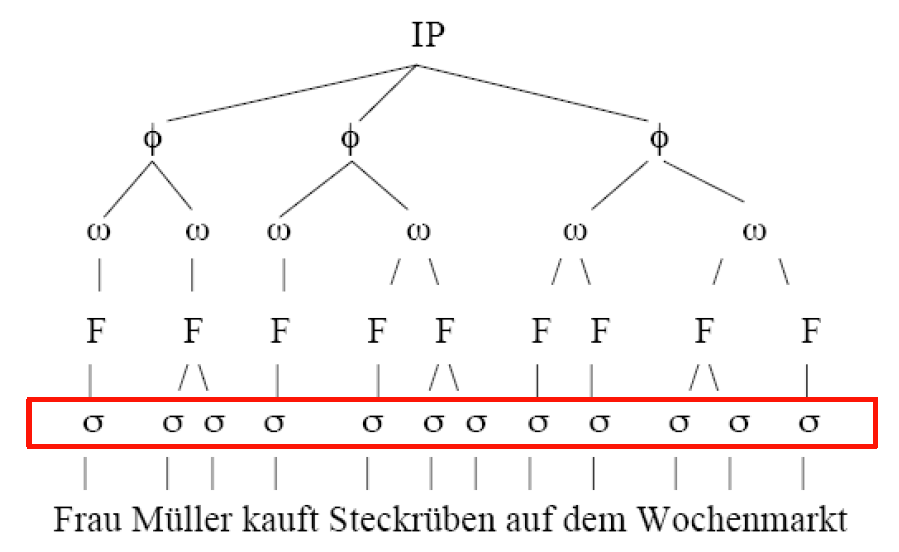
\includegraphics[scale=0.3]{material/03bHierarchieIntonationsphrase}
%	\caption{Hierarchie in der Intonationsphrase (Darstellung von C. Féry)}
%	\label{Zeichen1}
%\end{figure}

\end{frame}



%%%%%%%%%%%%%%%%%%%%%%%%%%%%%%%%%%%

\begin{frame}
%\frametitle{Einführung}


\begin{itemize}
	\item Prosodische Konstituenten:
	\begin{multicols}{2}
	\begin{itemize}
		\item UP = Äußerungsphrase
		\item IP = Intonationsphrase
		\item $\varphi$ = phonol. Phrase
\columnbreak
		\item $\omega$ = phonol. Wort
		\item F = phonol. Fuß
		\item \alertred{$\sigma$ = Silbe}
	\end{itemize}
	\end{multicols}
\end{itemize}

\begin{minipage}{0.39\textwidth}
	\begin{figure}
	\centering
	\scalebox{.65}{
		\begin{forest} MyP edges,
		[UP, name=up
		[IP, name=IP
		[$\varphi$[$\omega$[F[$\sigma$][$\sigma$]][F[$\sigma$][$\sigma$]]]]
		[$\varphi$, name=Phi[$\omega$[F[$\sigma$][$\sigma$]]][$\omega$, name=omega[F, name=F[$\sigma$][$\sigma$, name=sigma]]]]
		]]
		{\draw[black] (up.east)--(3.2,0);
			\draw[black] (IP.east)--(3.2,-1);
			\draw[black] (Phi.east)--(3.2,-2);
			\draw[black] (omega.east)--(3.2,-3);
			\draw[black] (F.east)--(3.2,-4);
			\draw[black] (sigma.east)--(3.2,-5.2);
	}
		\end{forest}
	}
		\caption{\cite{Fuhrhop&Co13a}}
	\end{figure}
\end{minipage}\hfill%
\begin{minipage}{0.6\textwidth}
	\footnotesize{(Mandarinen oder Äpfel)\textsubscript{UP}\\
	\\
	(Mandarinen oder Äpfel)\textsubscript{IP}\\
	\\
	(Mandarinen)\textsubscript{$\varphi$} (oder Äpfel)\textsubscript{$\varphi$}\\
	\\
	(Mandarinen)\textsubscript{$\omega$} (oder)\textsubscript{$\omega$} (Äpfel)\textsubscript{$\omega$}\\
	\\
	(Manda)\textsubscript{F} (rinen)\textsubscript{F} (oder)\textsubscript{F} (Äpfel)\textsubscript{F} \\
	\\
	(Man)\textsubscript{$\sigma$} (da)\textsubscript{$\sigma$} (ri)\textsubscript{$\sigma$} (nen)\textsubscript{$\sigma$} (o)\textsubscript{$\sigma$} (der)\textsubscript{$\sigma$} (Äp)\textsubscript{$\sigma$} (fel)\textsubscript{$\sigma$}
}
\vspace{1cm}
\end{minipage}


%\begin{figure}[b]
%	\centering
%	
%	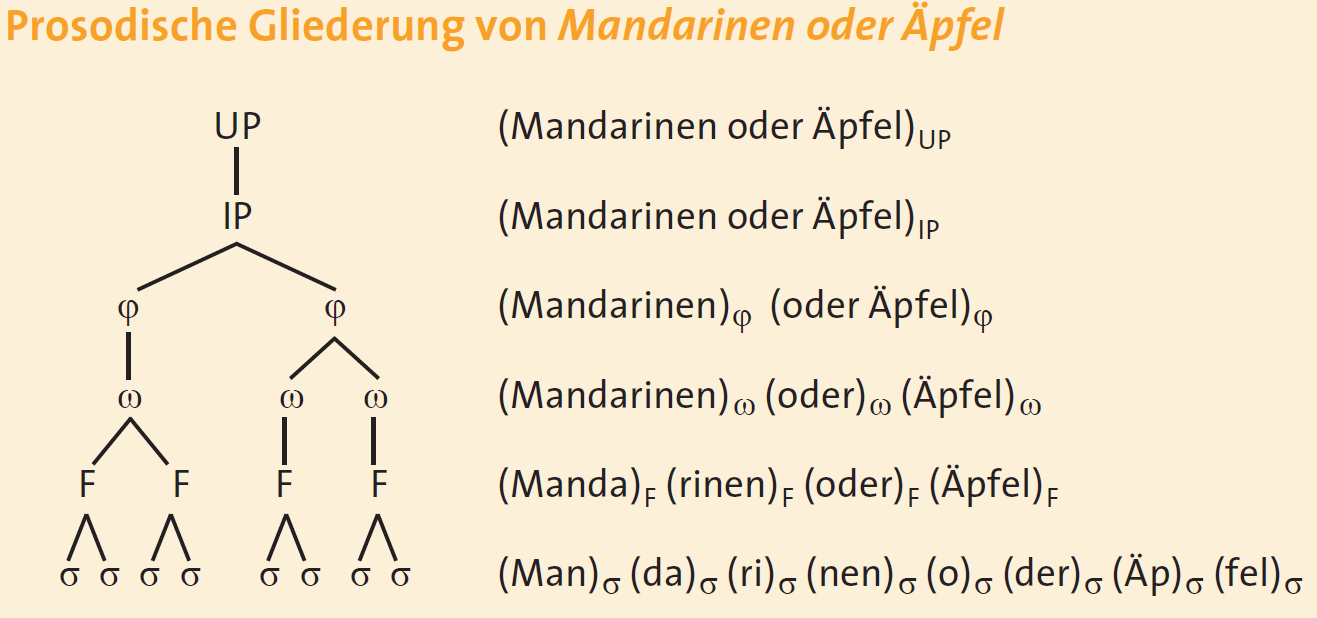
\includegraphics[scale=0.26]{material/03bHierarchieUP}
%	\caption{Hierarchie in der Äußerungsphrase \citep[8]{Fuhrhop&Co13a}}
%	%\label{Zeichen1}
%\end{figure}


\end{frame}



%%%%%%%%%%%%%%%%%%%%%%%%%%%%%%%%%%
%%%%%%%%%%%%%%%%%%%%%%%%%%%%%%%%%%
\subsection{Silbenbestimmung}
%\frame{
%\frametitle{~}
%\begin{multicols}{2}
%	\tableofcontents[currentsection]
%\end{multicols}	
%}
%%%%%%%%%%%%%%%%%%%%%%%%%%%%%%%%%%

\begin{frame}
\frametitle{Silbenbestimmung}

\begin{itemize}
	\item<1-> Wie viele Silben hat das folgende Wort?
	
	  \ea
          Silbenbestimmung
          \z
          
	
	\item<2-> Woher wissen Sie das?
	
	\begin{itemize}
		\item<2-> Staffeldt (2010: 133):\\
		\gqq{Jeder kompetente Sprachteilhaber verfügt über die \textbf{Fähigkeit}, Silben identifizieren zu können.}
		
		\item<2-> \citet[600]{Bussmann02a}:\\
		\gqq{Silbe: Phonetisch- phonologische \textbf{Grundeinheit} des Wortes bzw. der Rede, die zwar \textbf{intuitiv} nachweisbar ist, wissenschaftlich aber \textbf{nicht einheitlich definiert} wird.}
		
	\end{itemize}

	\item<2-> Silben können \textbf{betont} werden (tragen Akzent)
	
	\item<2-> Silbenspiele
% Geheimsprache, nach Silben wird immer pi, pa, pe oder so eingesetzt
	
	\item<2-> Intuitiv erkennbare Einheit

\end{itemize}

\end{frame}



%%%%%%%%%%%%%%%%%%%%%%%%%%%%%%%%%%
%%%%%%%%%%%%%%%%%%%%%%%%%%%%%%%%%%
\subsection{Silbenstruktur}
%\frame{
%\frametitle{~}
%\begin{multicols}{2}
%	\tableofcontents[currentsection]
%\end{multicols}	
%
%}
%%%%%%%%%%%%%%%%%%%%%%%%%%%%%%%%%%
\begin{frame}
\frametitle{Silbenstruktur}

\begin{itemize}
	\item Welche Silben (des Deutschen) sind mit den folgenden Segmenten bildbar?
	
	  \ea
          \textipa{[p]}, \textipa{[a]}, \textipa{[l]}, \textipa{[t]}
          \z
\pause	
\eal
\ex Bildbar:\\
	\textipa{[palt]}, \textipa{[alpt]}, \textipa{[lapt]}, \textipa{[talp]}, \textipa{[plat]}
\ex Nicht bildbar:\\
	*\textipa{[ltap]}, \\
	*\textipa{[lpat]},\\
	*\textipa{[ptla]}, \\
	*\textipa{[tpal]}, \dots \\
\zl
\pause
	\item Warum?
\end{itemize}

\end{frame}



%%%%%%%%%%%%%%%%%%%%%%%%%%%%%%%%%%%
%\begin{frame}
%\frametitle{Silbenstruktur}
%
%Die Silbe ist \textbf{intern strukturiert} und besteht aus den folgenden Teilen:
%
%\begin{minipage}{.60\textwidth}
%
%\begin{itemize}
%	\item[]
%	\item Silbenanlaut / Silbenanfangsrand / \alert{Onset},
%	\begin{itemize}
%		\item 0 bis $n$ Konsonanten, wobei in fast allen Sprachen $n < 5$
%	\end{itemize}
%	
%	\item[]
%	\item Silbengipfel / Silbenkern / \alert{Nukleus},
%	\begin{itemize}
%		\item Vokale
%		\item manchmal (vokalische) Nasale oder Liquide
%	\end{itemize}
%	
%	\item[]
%	\item Silbenauslaut / Silbenendrand / \alert{Koda}
%	\begin{itemize}
%		\item 0 bis $n$ Konsonanten, wobei in fast allen Sprachen $n < 5$
%	\end{itemize}
%
%	\item[]
%	\item Nukleus und Koda bilden den \alert{Reim}
%	
%\end{itemize}
%
%
%\end{minipage}
%\begin{minipage}{.39\textwidth}
%
%%%%%%%%%%%%%%
%%% Forestset Syllables

\newbox\foreststrutbox
\setbox\foreststrutbox=\hbox to 0pt{\phantom{\forestOve{standard node}{content}}}
\def\foreststrut{\copy\foreststrutbox}
\forestset{
GP1/.style 2 args={
for n={1}{baseline},
s sep=0pt, l sep=0pt,
for descendants={
l sep=0pt, l={#1},
anchor=base,calign=first,child anchor=north,
inner xsep=1pt,inner ysep=2pt,outer sep=0pt,s sep=0pt,
},
delay={
if content={}{phantom}{for children={no edge}},
for tree={
if content={O}{tier=OR}{},
if content={R}{tier=OR}{},
if content={N}{tier=N}{},
if content={x}{
tier=x,content={$\times$},outer xsep={#2},
for tree={calign=center},
for descendants={content format={\foreststrut\forestoption{content}}},
before drawing tree={outer xsep=0pt,delay={typeset node}},
s sep=4pt
}{},
},
},
before drawing tree={where content={}{parent anchor=center,child anchor=center}{}},
},
GP1/.default={5ex}{8.0pt},
associate/.style={%
tikz+={\draw(!)--(!#1);}},
spread/.style={
before drawing tree={tikz+={\draw[dotted](!)--(!#1);}}},
govern/.style={
before drawing tree={tikz+={\draw[->](!)--(!#1);}}},
p-govern/.style={
before drawing tree={tikz+={\draw[->](.north) to[out=150,in=30] (!#1.north);}}},
no p-govern/.style={
before drawing tree={tikz+={\draw[->,loosely dashed](.north) to[out=150,in=30] (!#1.north);}}},
encircle/.style={before drawing tree={circle,draw,inner sep=0pt}},
fen/.style={pin={[font=\footnotesize,inner sep=1pt,pin edge=<-]10:\textsc{Fen}}},
el/.style={content=\textsc{\textbf{##1}}},
head/.style={content=\textsc{\textbf{\underline{##1}}}},
llap/.style={
tikz+={%
\edef\forest@temp{\noexpand\node[\option{node options},
anchor=base east,at=(.base east)]}%
\forest@temp{#1\phantom{\option{environment}}};
}
},
rlap/.style={
tikz+={%
\edef\forest@temp{\noexpand\node[\option{node options},
anchor=base west,at=(.base west)]}%
\forest@temp{\phantom{\option{environment}}#1};
}
},
}
%%%%%%%%%%%%%

%\begin{figure}
%\centering
%\begin{forest} MyP edges, GP1 [
%  [$\sigma$
%    [O	[ [C$^{n}$]]
%    ]
%    [R	[N
%    		[V$^{n}$]
%    	]
%    	[K
%    		[C$^{n}$]
%    	]
%    ]
%  ]
%]
%\end{forest}
%\caption{Silbenstruktur}
%\end{figure}
%
%\end{minipage}
%
%\end{frame}



%%%%%%%%%%%%%%%%%%%%%%%%%%%%%%%%%%

\begin{frame}
%\frametitle{Silbenstruktur}

Die Silbe ist \textbf{intern strukturiert} und besteht aus den folgenden Teilen:

\begin{minipage}{.59\textwidth}

\begin{itemize}
	\item[]
	\item \alertred{Onset}
	
	\item \alertred{Reim}
	
	\item \alertred{Nukleus}
	
	\item \alertred{Koda}
	\item[] 
	\item C $:=$ Konsonantisch, d.\,h. nicht-silbisch ($\neq$Konsonant)
	\item V $:=$ Vokalisch, d.\,h. silbisch ($\neq$Vokal)
	
\end{itemize}


\end{minipage}
\begin{minipage}{.40\textwidth}

%%%%%%%%%%%%%%
%%% Forestset Syllables

\newbox\foreststrutbox
\setbox\foreststrutbox=\hbox to 0pt{\phantom{\forestOve{standard node}{content}}}
\def\foreststrut{\copy\foreststrutbox}
\forestset{
GP1/.style 2 args={
for n={1}{baseline},
s sep=0pt, l sep=0pt,
for descendants={
l sep=0pt, l={#1},
anchor=base,calign=first,child anchor=north,
inner xsep=1pt,inner ysep=2pt,outer sep=0pt,s sep=0pt,
},
delay={
if content={}{phantom}{for children={no edge}},
for tree={
if content={O}{tier=OR}{},
if content={R}{tier=OR}{},
if content={N}{tier=N}{},
if content={x}{
tier=x,content={$\times$},outer xsep={#2},
for tree={calign=center},
for descendants={content format={\foreststrut\forestoption{content}}},
before drawing tree={outer xsep=0pt,delay={typeset node}},
s sep=4pt
}{},
},
},
before drawing tree={where content={}{parent anchor=center,child anchor=center}{}},
},
GP1/.default={5ex}{8.0pt},
associate/.style={%
tikz+={\draw(!)--(!#1);}},
spread/.style={
before drawing tree={tikz+={\draw[dotted](!)--(!#1);}}},
govern/.style={
before drawing tree={tikz+={\draw[->](!)--(!#1);}}},
p-govern/.style={
before drawing tree={tikz+={\draw[->](.north) to[out=150,in=30] (!#1.north);}}},
no p-govern/.style={
before drawing tree={tikz+={\draw[->,loosely dashed](.north) to[out=150,in=30] (!#1.north);}}},
encircle/.style={before drawing tree={circle,draw,inner sep=0pt}},
fen/.style={pin={[font=\footnotesize,inner sep=1pt,pin edge=<-]10:\textsc{Fen}}},
el/.style={content=\textsc{\textbf{##1}}},
head/.style={content=\textsc{\textbf{\underline{##1}}}},
llap/.style={
tikz+={%
\edef\forest@temp{\noexpand\node[\option{node options},
anchor=base east,at=(.base east)]}%
\forest@temp{#1\phantom{\option{environment}}};
}
},
rlap/.style={
tikz+={%
\edef\forest@temp{\noexpand\node[\option{node options},
anchor=base west,at=(.base west)]}%
\forest@temp{\phantom{\option{environment}}#1};
}
},
}
%%%%%%%%%%%%%


\begin{figure}
\centering
\begin{forest} MyP edges, GP1 [
  [$\sigma$
    [O
    	[[C[\textipa{S}]]]
    	[[C[\textipa{t}]]]
    	[[C[\textipa{\textscr}]]]
    ]
    [R
    	[N
    		[V[\textipa{U}]]
    	]
    	[K
    		[C[\textipa{m}]]
    		[C[\textipa{\t{pf}}]]
    		[C[\textipa{s}]]
    		[C[\textipa{t}]]
    	]
    ]
  ]
]
\end{forest}
\caption{Komplexe Silbe}
\end{figure}
% wahrscheinlich komplexeste Koda, die es gibt.
\end{minipage}

\end{frame}



%%%%%%%%%%%%%%%%%%%%%%%%%%%%%%%%%%
\begin{frame}
%\frametitle{Silbenstruktur}

Die Silbe ist \textbf{intern strukturiert} und besteht aus den folgenden Teilen:

\begin{minipage}{.60\textwidth}

\begin{itemize}
	\item[]
	\item \alertred{Onset}
	
	\item \alertred{Reim}
	
	\item \alertred{Nukleus}
	
	\item \alertred{Koda}
	\item[] 
	\item \textbf{Minimale Silbe} besteht nur aus einem V im  Nukleus
	  \ea
          \ab{gehe} \ras \textipa{[ge:.@]}
          \z
	
\end{itemize}


\end{minipage}
\begin{minipage}{.39\textwidth}

%%%%%%%%%%%%%%
%%% Forestset Syllables

\newbox\foreststrutbox
\setbox\foreststrutbox=\hbox to 0pt{\phantom{\forestOve{standard node}{content}}}
\def\foreststrut{\copy\foreststrutbox}
\forestset{
GP1/.style 2 args={
for n={1}{baseline},
s sep=0pt, l sep=0pt,
for descendants={
l sep=0pt, l={#1},
anchor=base,calign=first,child anchor=north,
inner xsep=1pt,inner ysep=2pt,outer sep=0pt,s sep=0pt,
},
delay={
if content={}{phantom}{for children={no edge}},
for tree={
if content={O}{tier=OR}{},
if content={R}{tier=OR}{},
if content={N}{tier=N}{},
if content={x}{
tier=x,content={$\times$},outer xsep={#2},
for tree={calign=center},
for descendants={content format={\foreststrut\forestoption{content}}},
before drawing tree={outer xsep=0pt,delay={typeset node}},
s sep=4pt
}{},
},
},
before drawing tree={where content={}{parent anchor=center,child anchor=center}{}},
},
GP1/.default={5ex}{8.0pt},
associate/.style={%
tikz+={\draw(!)--(!#1);}},
spread/.style={
before drawing tree={tikz+={\draw[dotted](!)--(!#1);}}},
govern/.style={
before drawing tree={tikz+={\draw[->](!)--(!#1);}}},
p-govern/.style={
before drawing tree={tikz+={\draw[->](.north) to[out=150,in=30] (!#1.north);}}},
no p-govern/.style={
before drawing tree={tikz+={\draw[->,loosely dashed](.north) to[out=150,in=30] (!#1.north);}}},
encircle/.style={before drawing tree={circle,draw,inner sep=0pt}},
fen/.style={pin={[font=\footnotesize,inner sep=1pt,pin edge=<-]10:\textsc{Fen}}},
el/.style={content=\textsc{\textbf{##1}}},
head/.style={content=\textsc{\textbf{\underline{##1}}}},
llap/.style={
tikz+={%
\edef\forest@temp{\noexpand\node[\option{node options},
anchor=base east,at=(.base east)]}%
\forest@temp{#1\phantom{\option{environment}}};
}
},
rlap/.style={
tikz+={%
\edef\forest@temp{\noexpand\node[\option{node options},
anchor=base west,at=(.base west)]}%
\forest@temp{\phantom{\option{environment}}#1};
}
},
}
%%%%%%%%%%%%%


\begin{figure}
\centering
\begin{forest} MyP edges, GP1 [
  [$\sigma$
    [O
    ]
    [R
    	[N
    		[V[\textipa{@}]]
    	]
    	[K
    	]
    ]
  ]
]
\end{forest}
\caption{Minimale Silbe}
\end{figure}


\end{minipage}

\end{frame}

%%%%%%%%%%%%%%%%%%%%%%%%%%%%%%%%%%
\begin{frame}
%\frametitle{Silbenstruktur}

\begin{itemize}
	\item Silbenanlaut/Silbenanfangsrand/\alertred{Onset},
	\item Silbengipfel/Silbenkern/\alertred{Nukleus},
	\item Silbenauslaut/Silbenendrand/\alertred{Koda}
	
\end{itemize}

\begin{table}
\centering
\begin{tabular}{lllll}
\textsc{Onset} & \textsc{Nukleus} & \textsc{Koda} & \textsc{Term} & \textsc{Merkmal} \\
\hline
\textipa{z} & \textipa{e:} & & Offene Silbe & Koda leer\\
\hline
\textipa{t} & \textipa{a:} & \textipa{l} & Geschlossene Silbe & Koda besetzt\\
\hline
 & \textipa{@} & \textipa{n} & Nackte Silbe & Onset leer\\
\hline
\textipa{z} & \textipa{e:} & & Bedeckte Silbe & Onset besetzt\\
\end{tabular}
\end{table}

\end{frame}



%%%%%%%%%%%%%%%%%%%%%%%%%%%%%%%%%%
%%%%%%%%%%%%%%%%%%%%%%%%%%%%%%%%%%
%\subsubsection{Onset}
%\frame{
%\begin{multicols}{2}
%\frametitle{~}
%	\tableofcontents[currentsection]
%\end{multicols}
%}
%%%%%%%%%%%%%%%%%%%%%%%%%%%%%%%%%%

\begin{frame}
\frametitle{Onset}

\begin{multicols}{2}
Sprachbeispiele:
	
\ea
Tschechisch \textipa{[fspla.nout]} \gq{aufflammen}
\z

\ea
Hawaianisch \textipa{[a.lo.ha]} \gq{Liebe}
\z

\ea
Deutsch \textipa{[St\textscr aIt]} \gq{Streit}
\z

Im Deutschen sind
	\begin{itemize}
		\item \textbf{3 Cs} beschränkt möglich (nach \textipa{/S/} und \textipa{/s/}),

% 3 = Streit, häfiger 2
		
		\item \textbf{2 Cs} oft (\zB \textipa{/bl/}, \textipa{/kn/} \dots\ ), und
		\item \textbf{1 C} immer (bis auf \textipa{[N]})
	\end{itemize}

\columnbreak

\begin{table}
\centering

\begin{tabular}{c|c|c|c|c}
 & \textipa{m} & \textipa{n} & \textipa{l} & \textipa{\textscr} \\ 
\hline 
\textipa{p} &  &  & + & + \\ 
\hline 
\textipa{b} &  &  & + & + \\ 
\hline 
\textipa{t} &  &  &  & + \\ 
\hline 
\textipa{d} &  &  &  & + \\ 
\hline 
\textipa{k} &  & + & + & + \\ 
\hline 
\textipa{g} &  & + & + & + \\ 
\hline 
\textipa{f} &  &  & + & + \\
\hline 
\textipa{v} &  &  &  & + \\ 
\hline 
\textipa{S} & + & + & + & + \\ 
\end{tabular} 

\caption{Kombinatorik}
\end{table}

\end{multicols}

\end{frame}



%%%%%%%%%%%%%%%%%%%%%%%%%%%%%%%%%%

\begin{frame}
%\frametitle{Onset}

\begin{itemize}
	\item Bei Betrachtung aller (bekannten) Sprachen kann man die folgende Gesetzmäßigkeit feststellen \citep[cf.][212f.]{Hall00a}
	
	\begin{block}{Silbenanlautgesetz}
	
	\sub{$\sigma$}[CV $>$ \sub{$\sigma$}[V 
	und
	\sub{$\sigma$}[C\MyPup{$n$}V $>$ \sub{$\sigma$}[C\MyPup{$n+1$}V \\
	$>$ $:=$ häufiger als oder ist weniger markiert als 

% Silbe mit Konsonant und Vokal sind häfiger als solche, die nur mit Vokal beginnen
% Silbe mit n Konsonanten ist weniger markiert als Silbe mit n+1 KOnsonanten.


	
	\end{block}
	 
	 \item Man spricht auch von der Markiertheit von Silben, wenn sie Präferenzgesetzen widersprechen.

\end{itemize}

\end{frame}



%%%%%%%%%%%%%%%%%%%%%%%%%%%%%%%%%%
%%%%%%%%%%%%%%%%%%%%%%%%%%%%%%%%%%
%\subsubsection{Nukleus}
%\frame{
%\begin{multicols}{2}
%\frametitle{~}
%	\tableofcontents[currentsection]
%\end{multicols}
%}
%%%%%%%%%%%%%%%%%%%%%%%%%%%%%%%%%%

\begin{frame}
\frametitle{Nukleus}

\begin{itemize}

	\item In allen Sprachen werden Nuklei durch \textbf{Vokale} (V) gebildet
	
	\item In einigen Sprachen können Nuklei auch durch \textbf{Liquide und Nasale} (C \ras V) gebildet werden


	
	\item Im Deutschen werden bei schnellem Sprechen folgende Wörter mit so genannten \textbf{silbischen Konsonanten} gesprochen
	
	
          \ea
          \ab{lesen} \textipa{[le:.z\textsyllabic{n}]} %
          \z
          
          \ea
          \ab{Wandel} \textipa{[van.d\textsyllabic{l}]}
          \z

	\item Bei Betrachtung aller (bekannten) Sprachen kann man die folgende Gesetzmäßigkeit feststellen \citep[cf.][217f.]{Hall00a}

\end{itemize}
	
	\begin{block}{Silbenkerngesetz}
	
	Silben mit einfachem vokalischem Nukleus sind universell bevorzugt.
	
	Vokale $>$ Sonoranten $>$ Obstruenten 
	
	\end{block}
	
\end{frame}



%%%%%%%%%%%%%%%%%%%%%%%%%%%%%%%%%%
%%%%%%%%%%%%%%%%%%%%%%%%%%%%%%%%%%
%\subsubsection{Koda}
%\frame{
%\begin{multicols}{2}
%\frametitle{~}
%	\tableofcontents[currentsection]
%\end{multicols}
%}
%%%%%%%%%%%%%%%%%%%%%%%%%%%%%%%%%%

\begin{frame}
\frametitle{Koda}

In der Koda sind/ist \dots

\begin{itemize}

	\item \dots\ in \emph{vielen} Sprachen keine Konsonanten erlaubt (\zB Hawaiianisch),
	
	\item \dots\ in \emph{einigen} Sprachen ein Konsonant erlaubt,
	
	\item \dots\ in \emph{einigen (wenigen)} Sprachen mehrere Konsonanten erlaubt.
	
	\item[]
	\item Deutsch: \textipa{[hE\textscr psts]} (0 bis 4/5 Konsonanten)
	
	\item Reihenfolge der Konsonanten unterliegt dem  \textbf{Sonoritätsprinzip}
	
	\item Bei Betrachtung aller (bekannten) Sprachen kann man die folgende Gesetzmäßigkeit feststellen \citep[cf.][214]{Hall00a}

\end{itemize}
	
	\begin{block}{Silbenauslautgesetz}
	
	CVC$^{n}$]$_{\sigma}$ $>$ CVC$^{n+1}$]$_{\sigma}$
	
	\end{block}
	
\end{frame}



%%%%%%%%%%%%%%%%%%%%%%%%%%%%%%%%%%%
%%%%%%%%%%%%%%%%%%%%%%%%%%%%%%%%%%%
\subsection{Phonotaktik}
\iftoggle{toc}{
\frame{
\frametitle{~}
\begin{multicols}{2}
	\tableofcontents[currentsection]
\end{multicols}	
}
}
%%%%%%%%%%%%%%%%%%%%%%%%%%%%%%%%%%

\begin{frame}
\frametitle{Phonotaktik}

\begin{block}{Phonotaktik}

Die Phonotaktik untersucht die syntagmatischen Beziehungen zwischen Lauten innerhalb der Silbe und anderer prosodischer Einheiten \citep{Fuhrhop&Co13a}

\end{block}

\begin{itemize}
	\item Mögliche und unmögliche Kombinationen von Segmenten bzgl.
	
	\begin{itemize}
		\item Anzahl der Laute,
		\item Art,
		\item Reihenfolge der Laute
	\end{itemize}

\end{itemize}

\end{frame}



%%%%%%%%%%%%%%%%%%%%%%%%%%%%%%%%%%%
%%%%%%%%%%%%%%%%%%%%%%%%%%%%%%%%%%%
%\subsubsection{Sonoritätshierarchie}
%\frame{
%\begin{multicols}{2}
%\frametitle{~}
%	\tableofcontents[currentsection]
%\end{multicols}
%}
%%%%%%%%%%%%%%%%%%%%%%%%%%%%%%%%%%

\begin{frame}
\frametitle{Sonoritätshierarchie}

\begin{itemize}
	\item Betrachten Sie die folgenden Beispiele und überlegen Sie \dots
	
	\begin{enumerate}
		\item \dots\ welche \textbf{phonotaktischen Beschränkungen} für den Onset in deutschen Silben gelten könnten:

                  \ea
                  \textipa{[\textcolor{red}{k\textscr}aNk]}, \textipa{[\textcolor{red}{pl}a:n]}, \textipa{[\textcolor{red}{f\textscr} E\c{c}]},
                  \textipa{[\textcolor{red}{fl}o:]}, \textipa{[\textcolor{red}{kn}i:]}, \textipa{[\textcolor{red}{gn}a:d@]}
                  \z

                  \ea
                  *\textipa{[\textcolor{red}{{\textscr}k}aNk]}, *\textipa{[\textcolor{red}{lp}a:n]}, *\textipa{[\textcolor{red}{{\textscr}f}E\c{c}]}, *\textipa{[\textcolor{red}{lf}o:]}, *\textipa{[\textcolor{red}{nk}i:]}, *\textipa{[\textcolor{red}{ng}a:d@]}
                  \z
                  
\pause
		\item \dots\ welche \textbf{phonotaktischen Beschränkungen} für die Koda in deutschen Silben gelten könnten:

                  \ea
                  \textipa{[ka\textcolor{red}{lt}]}, \textipa{[ha\textcolor{red}{{\textscr}t}]}, \textipa{[la\textcolor{red}{nt}]}, \textipa{[k{\textscr}a\textcolor{red}{Nk}]}
                  \z

                  \ea
                  *\textipa{[ka{tl}]}, *\textipa{[ha{t\textscr}]}, *\textipa{[la\textcolor{red}{tn}]},
                  *\textipa{[k\textscr a\textcolor{red}{kN}]}
                  \z

	\end{enumerate}
	
\end{itemize}

\end{frame}



%%%%%%%%%%%%%%%%%%%%%%%%%%%%%%%%%%
\begin{frame}
%\frametitle{Sonoritätshierarchie}

\begin{enumerate}
	\item \textbf{phonotaktischen Beschränkungen} \ras Onset
	
          \ea
          \textipa{[k\textscr aNk]}, \textipa{[pla:n]}, \textipa{[f\textscr E\c{c}]},
          \textipa{[flo:]}, \textipa{[kni:]}, \textipa{[gna:d@]}
          \z

          \ea
          *\textipa{[lbat]}, *\textipa{[\textscr to:k]}, *\textipa{[nki:l]}, *\textipa{[ngak]}
          \z

	\item \textbf{phonotaktischen Beschränkungen} \ras Koda

          \ea
          \textipa{[kalt]}, \textipa{[ha5t]}, \textipa{[lant]}, \textipa{[k\textscr aNk]}
          \z

          \ea
          *\textipa{[katl]}, *\textipa{[hat\textscr ]}, *\textipa{[latn]}, *\textipa{[k\textscr
              akN]}
          \z

\end{enumerate}
	

\begin{table}
\centering
\begin{tabular}{c|c|c|c|c} 
 & Sonorant & Obstruent & Vokal & Laryngal \\ 
\hline 
[kon] & $[+]$ & $[+]$ & $[-]$ & $[-]$ \\ 
\hline 
[son] & $[+]$ & $[-]$ & $[+]$ & $[-]$
\end{tabular} 

\end{table}

\begin{itemize}
	\item \textbf{Onset}: Obstruent vor Sonorant
	\item \textbf{Koda}: Sonorant vor Obstruent
\end{itemize}

\end{frame}



%%%%%%%%%%%%%%%%%%%%%%%%%%%%%%%%%%

\begin{frame}
%\frametitle{Sonoritätshierarchie}

\begin{itemize}
	\item Eine Silbe ist so aufgebaut, dass die Sonorität in der Silbe zum Nukleus hin steigt und dann abfällt.

	\item \textbf{Sonorität} $:=$ Schallfülle, Intensität

\end{itemize}

\begin{figure}
\centering
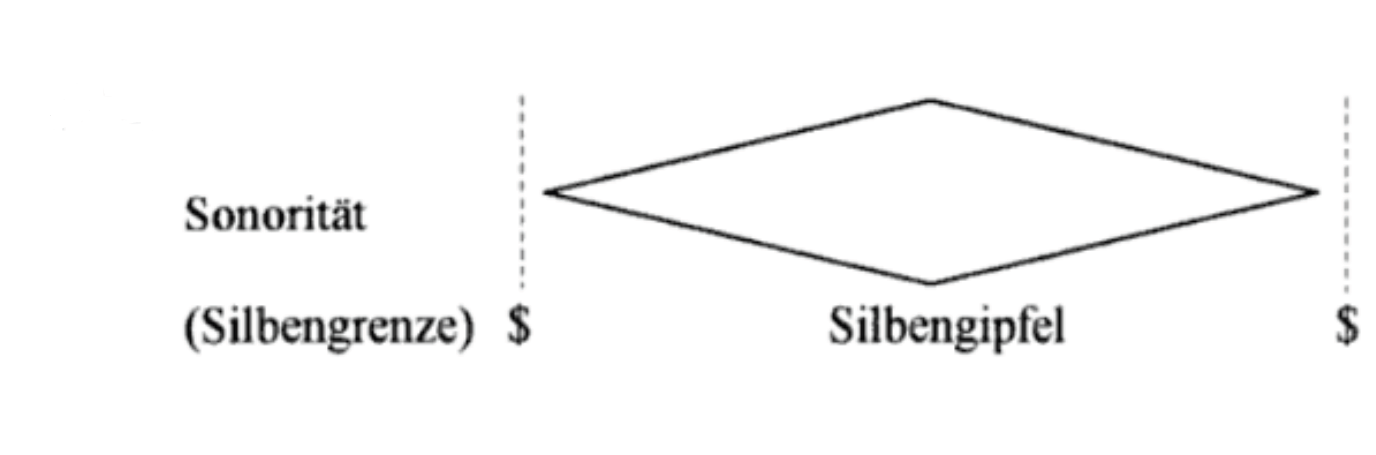
\includegraphics[scale=.2]{material/03bSonoritaetRamers}
\caption{Nach \citet[93]{Ramers08a} (apud Lenerz 1985)}
\end{figure}
% Vokale sind sonorste Elemente
% m > p

% s > p  (frikativ > plosiv)

\begin{itemize}
	\item Laute können nach der Sonoritätshierarchie auf einer Skala (nach ihrer \textbf{Sonorität}) angeordnet werden.
\end{itemize}

\end{frame}



%%%%%%%%%%%%%%%%%%%%%%%%%%%%%%%%%%

\begin{frame}
%\frametitle{Sonoritätshierarchie}

\begin{itemize}
	\item Es gibt verschiedene Ausformulierungen der Sonoritätshierachie.

\end{itemize}

\begin{table}
\centering
\begin{tabular}{l|l|l|l|l} 
	 & einfach 				  	 & Hall 					  & \textbf{Wiese} 				& komplex  \\ 
\hline
\hline 
$[+]$& \multirow{6}{*}{Sonorant} & \multirow{2}{*}{Vokal} 	  & \multirow{2}{*}{Vokal} 		& Vokal  \\ 
	 & 							 & 						 	  &								& Vokal (hoch) \\
\cline{3-5}			
	 &							 & \multirow{3}{*}{Liquide}   &								& Gleitlaut \\
	 &						  	 &	 						  & \textipa{/\textscr /}		& Vibrant \\
\cline{4-5}			
	 &						 	 &							  & \textipa{/l/}				& Lateral \\
\cline{3-5}			
	 &							 & Nasal					  & Nasal						& Nasal \\
\hline			
	 &\multirow{6}{*}{Obstruent} & \multirow{6}{*}{Obstruent} & \multirow{3}{*}{Frikativ}	& $[+$sth$]$ Frikativ \\
	 &						 	 &							  &								& $[+$sth$]$ Affrikat \\		
	 &							 &							  &								& $[+$sth$]$ Plosiv \\
\cline{4-5}			
	 &						  	 &							  & \multirow{3}{*}{Plosiv}		& $[-$sth$]$ Frikativ \\
	 &						 	 &							  &								& $[-$sth$]$ Affrikat \\		
$[-]$&							 &							  &								& $[-$sth$]$ Plosiv \\
		
\end{tabular} 

\end{table}

\end{frame}



%%%%%%%%%%%%%%%%%%%%%%%%%%%%%%%%%%

\begin{frame}
%\frametitle{Sonoritätshierarchie}


\begin{block}{Sonoritätsprinzip (Sonority Sequencing Generalization -- SSG)}
In jeder Silbe gibt es ein Segment, das den Silbengipfel bildet, und dem ein oder mehrere Segmente vorangehen und/oder folgen, deren Sonoritätswerte zum Silbengipfel hin zunehmen und danach abnehmen. (vgl. \citealt[225]{Hall00a}, \citealt[94]{Ramers08a})
\end{block}

\begin{itemize}
	\item Strikt: Monoton steigend oder fallend
	\item Abgeschwächt: auch gleichbleibend \citep[vgl.][]{Hall00a}

\end{itemize}

\begin{figure}
\centering
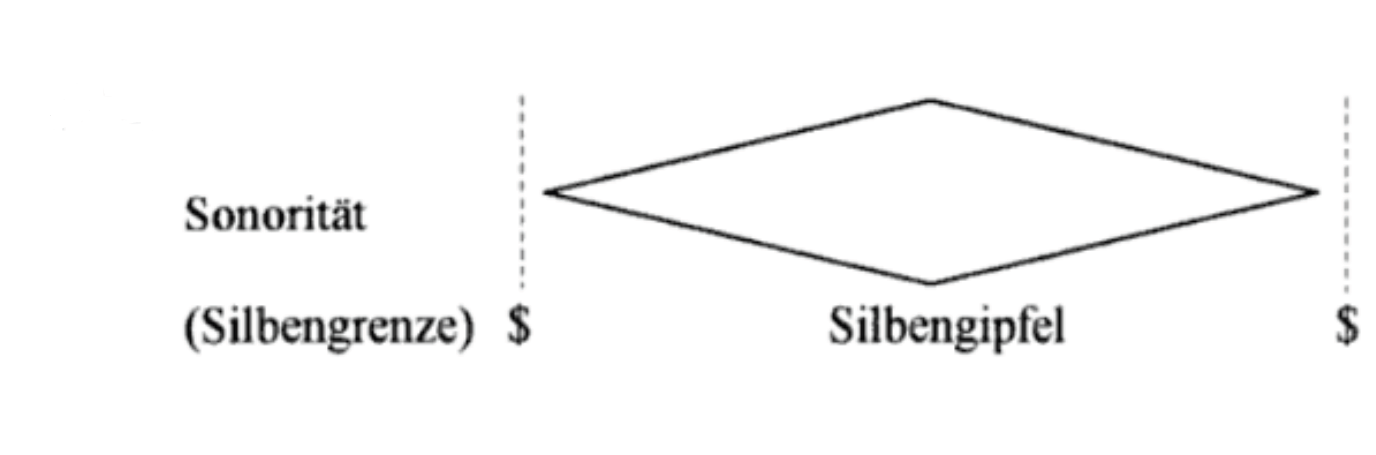
\includegraphics[scale=.2]{material/03bSonoritaetRamers}
\caption{Nach \citet[93]{Ramers08a} (apud Lenerz 1985)}
\end{figure}

\end{frame}



%%%%%%%%%%%%%%%%%%%%%%%%%%%%%%%%%%

\begin{frame}
%\frametitle{Sonoritätshierarchie}

\begin{block}{Sonoritätshierarchie (für uns)}
Vokal $>$ \textipa{/\textscr /} $>$ \textipa{/l/} $>$ Nasal $>$ Frikativ $>$ Plosiv \\
$x > y$ $:=$ $x$ ist sonorer als $y$
\end{block}

\begin{figure}
	\centering
	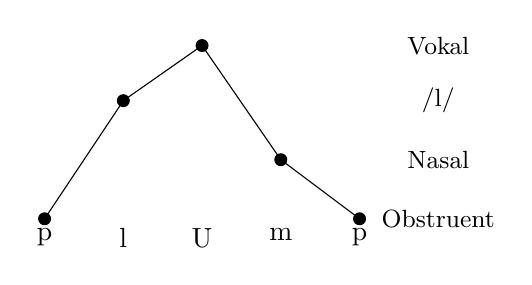
\begin{tikzpicture}
	\draw[fill] (0,0) circle [radius=0.075];
	\draw[black] (0,0)--(1,1.5);
	\draw[fill] (1,1.5) circle [radius=0.075];
	\draw[black] (1,1.5)--(2,2.2);
	\draw[fill] (2,2.2) circle [radius=0.075];
	\draw[black] (2,2.2)--(3,0.75);
	\draw[fill] (3,0.75) circle [radius=0.075];
	\draw[black] (3,0.75)--(4,0);
	\draw[fill] (4,0) circle [radius=0.075];
	\node[below] at (0,0){p};
	\node[below] at (1,0){l};
	\node[below] at (2,0){\textipa{U}};
	\node[below] at (3,0){m};
	\node[below] at (4,0){p};
	\node at (5,2.2){{\small Vokal}};
	\node at (5,1.5){{\small /l/}};
	\node at (5,0.75){{\small Nasal}};
	\node at (5,0){{\small Obstruent}};
\end{tikzpicture}
\caption{\citet[225]{Hall00a}}
\end{figure}


%\begin{figure}
%\centering
%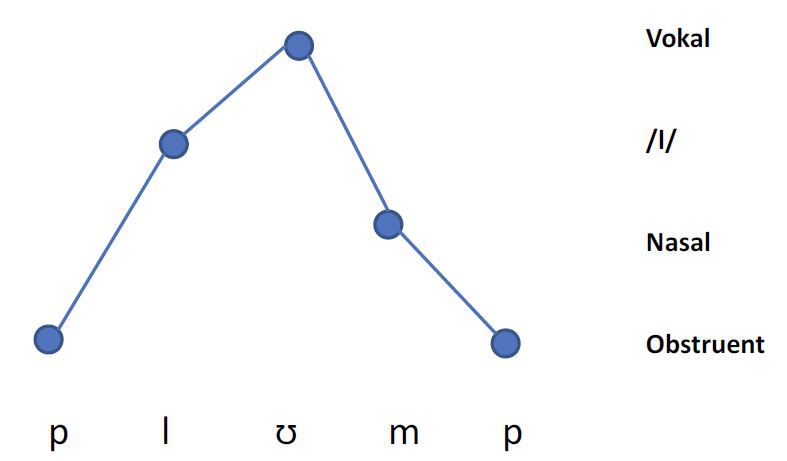
\includegraphics[scale=.3]{material/03bSonoritaetBsp}
%\caption{\citet[225]{Hall00a}}
%\end{figure}

\begin{itemize}
	\item Sonoritätshierarchie wird je nach Sprache leicht anders spezifiziert.
\end{itemize}
\end{frame}


\iftoggle{uebung}{
%%%%%%%%%%%%%%%%%%%%%%%%%%%%%%%%%%
\begin{frame}
\frametitle{Übung}

\begin{itemize}
	\item Geben Sie die Sonoritätsprofile der folgenden Silben an.
	
	  \ea
          Spatz, Dachs, Clown, Milch
          \z

% bei Spatz geht es von Frikativ s auf Plosiv p runter = Ausnahme
% bei Dachs geht es auf k runter und dann auf s hoch   = Ausnahme
% clown k = plosiv, l = /l/ au = Vokal, n = , keine Ausnahme

% Glottal stop gehört zu den Plosiven

	\item Erklären Sie die Ungramatikalität der folgenden Silben:
	
	  \ea
          *\textipa{[lbat]}, *\textipa{[blabl]}, *\textipa{[m{\textscr}apt]}, *\textipa{[ki:l\textscr]}, *\textipa{[ngang]}
          \z

% hier Probleme im Onset
% l sonorer als b


	\ea *\textipa{[krafm]}, *\textipa{[elat]}, *\textipa{[plaml]}, *\textipa{[nfatl]}

% hier auch Probleme in der Koda

        \z

\end{itemize}

\end{frame}
}

\iftoggle{loesung}{
	\begin{frame}
\frametitle{Lösung}

\begin{minipage}{.4\textwidth}
		\begin{figure}
		\centering
		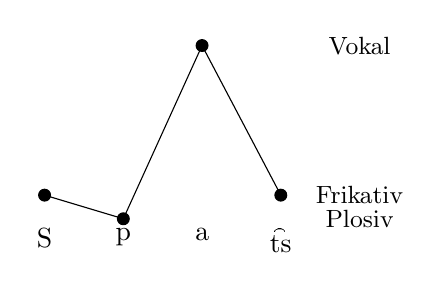
\begin{tikzpicture}
		\draw[fill] (0,0.3) circle [radius=0.075];
		\draw[black] (0,0.3)--(1,0);
		\draw[fill] (1,0) circle [radius=0.075];
		\draw[black] (1,0)--(2,2.2);
		\draw[fill] (2,2.2) circle [radius=0.075];
		\draw[black] (2,2.2)--(3,0.3);
		\draw[fill] (3,0.3) circle [radius=0.075];
		\node[below] at (0,0){\textipa{S}};
		\node[below] at (1,0){\textipa{p}};
		\node[below] at (2,0){\textipa{a}};
		\node[below] at (3,0){\textipa{\t{ts}}};
		\node at (4,0.3){{\small Frikativ}};
		\node at (4,0){{\small Plosiv}};
		\node at (4,2.2){{\small Vokal}};
		\end{tikzpicture}
	\end{figure}
\end{minipage}
\begin{minipage}{.1\textwidth}
	\hfill
\end{minipage}
\begin{minipage}{.4\textwidth}
		\begin{figure}
		\centering
		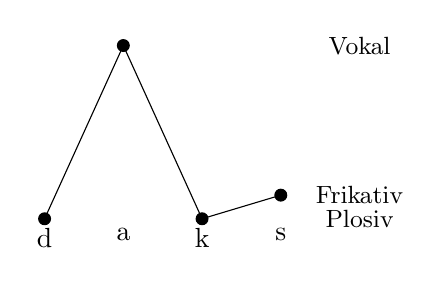
\begin{tikzpicture}
		\draw[fill] (0,0) circle [radius=0.075];
		\draw[black] (0,0)--(1,2.2);
		\draw[fill] (1,2.2) circle [radius=0.075];
		\draw[black] (1,2.2)--(2,0);
		\draw[fill] (2,0) circle [radius=0.075];
		\draw[black] (2,0)--(3,0.3);
		\draw[fill] (3,0.3) circle [radius=0.075];
		\node[below] at (0,0){\textipa{d}};
		\node[below] at (1,0){\textipa{a}};
		\node[below] at (2,0){\textipa{k}};
		\node[below] at (3,0){\textipa{s}};
		\node at (4,0.3){{\small Frikativ}};
		\node at (4,0){{\small Plosiv}};
		\node at (4,2.2){{\small Vokal}};
		\end{tikzpicture}
	\end{figure}
\end{minipage}

\begin{minipage}{.4\textwidth}
	\begin{figure}
		\centering
		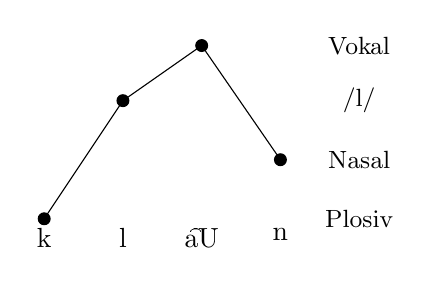
\begin{tikzpicture}
		\draw[fill] (0,0) circle [radius=0.075];
		\draw[black] (0,0)--(1,1.5);
		\draw[fill] (1,1.5) circle [radius=0.075];
		\draw[black] (1,1.5)--(2,2.2);
		\draw[fill] (2,2.2) circle [radius=0.075];
		\draw[black] (2,2.2)--(3,0.75);
		\draw[fill] (3,0.75) circle [radius=0.075];
		\node[below] at (0,0){\textipa{k}};
		\node[below] at (1,0){\textipa{l}};
		\node[below] at (2,0){\textipa{\t{aU}}};
		\node[below] at (3,0){\textipa{n}};
		\node at (4,1.5){{\small /l/}};
		\node at (4,0){{\small Plosiv}};
		\node at (4,2.2){{\small Vokal}};
		\node at (4,0.75){{\small Nasal}};
		\end{tikzpicture}
	\end{figure}
\end{minipage}
\begin{minipage}{.1\textwidth}
	\hfill
\end{minipage}
\begin{minipage}{.4\textwidth}
	\begin{figure}
		\centering
		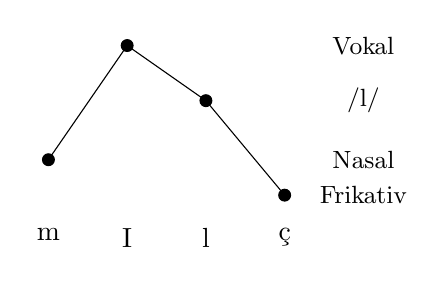
\begin{tikzpicture}
		\draw[fill] (0,0.75) circle [radius=0.075];
		\draw[black] (0,0.75)--(1,2.2);
		\draw[fill] (1,2.2) circle [radius=0.075];
		\draw[black] (1,2.2)--(2,1.5);
		\draw[fill] (2,1.5) circle [radius=0.075];
		\draw[black] (2,1.5)--(3,0.3);
		\draw[fill] (3,0.3) circle [radius=0.075];
		\node[below] at (0,0){\textipa{m}};
		\node[below] at (1,0){\textipa{I}};
		\node[below] at (2,0){\textipa{l}};
		\node[below] at (3,0){\textipa{\c{c}}};
		\node at (4,0.3){{\small Frikativ}};
		\node at (4,1.5){{\small /l/}};
		\node at (4,2.2){{\small Vokal}};
		\node at (4, 0.75){\small Nasal};
		\end{tikzpicture}
	\end{figure}
\end{minipage}

\end{frame}

\begin{frame}
	\frametitle{Lösung}
	\begin{itemize}
		\item \textipa{[bla\textcolor{red}{bl}]} \ras + Auslautverhärtung
		\item \textipa{[\textcolor{red}{ng}a\textcolor{red}{ng}]} \ras + Regressive velare Nasalassimilation + g-Tilgung
		\item \textipa{[\textcolor{red}{el}at]} \ras + Knacklauteinsetzung
	\end{itemize}
\end{frame}
}
%%%%%%%%%%%%%%%%%%%%%%%%%%%%%%%%%%
%%%%%%%%%%%%%%%%%%%%%%%%%%%%%%%%%%
%\subsubsection{Weitere phonotaktische Beschränkungen}
%\frame{
%\frametitle{~}
%\begin{multicols}{2}
%	\tableofcontents[currentsection]
%\end{multicols}	
%}
%%%%%%%%%%%%%%%%%%%%%%%%%%%%%%%%%%

\begin{frame}
\frametitle{Weitere phonotaktische Beschränkungen}

\begin{itemize}
	\item Im \textbf{Onset} in deutschen Silben können stehen:

	\begin{itemize}
		\item alle Einzelkonsonanten des Deutschen,
		\item außer \textipa{[s]} vor V, und \textipa{[N]}
		\item[]
		\item bestimmte zwei- und dreigliedrige Konsonantencluster (nach Sonoritätshierarchie)
	\end{itemize}
	
	\item[]

	\item Silben können auch \textbf{mit unbetontem Vokal} beginnen.

	\begin{itemize}
		\item Dann ist der Onset leer.
		  \ea
                  \textipa{[\textprimstress P\t{aɪ}.5]} (Eier)
                  \z

		  \ea
                  \textipa{[PEt.\textprimstress va:.I\c{c}]} (etwaig)
                  \z
	
	\end{itemize}
	
	\item Vor betontem Vokal steht immer der \textbf{Glottisschlag}.

	  \ea
          \textipa{[ka.\textprimstress Po:.tIS]}
          \z

\end{itemize}

\end{frame}



%%%%%%%%%%%%%%%%%%%%%%%%%%%%%%%%%%
%%%%%%%%%%%%%%%%%%%%%%%%%%%%%%%%%%
\subsection{Silbenmodelle}
\iftoggle{toc}{
\frame{
\frametitle{~}
\begin{multicols}{2}
	\tableofcontents[currentsection]
\end{multicols}	
}
}
%%%%%%%%%%%%%%%%%%%%%%%%%%%%%%%%%%

\begin{frame}
\frametitle{Silbenmodelle}

\begin{itemize}
	\item Bisher (hauptsächlich) nur \textbf{lineare Betrachtung} mit allen Segmenten auf einer Schicht
	  \ea
          \textipa{/pe:.t@\textscr /} (Peter)
          \z
	
	  \ea
          \textipa{/vE\.t@\textscr /} (Vetter)
          \z

	\item \textbf{Nicht-lineare Phonologie} (Autosegmentale Phonologie)
	
	\begin{itemize}
		\item verschiedene Repräsentationsebenen bzw. Schichten
		
		\item hierarchische Strukturierung
		
		\item Vorteil: Beschreibung von \textbf{Merkmalsausbreitung} und \textbf{segmentunabhängigen Prozessen}
		
	\end{itemize}
\end{itemize}

\end{frame}



%%%%%%%%%%%%%%%%%%%%%%%%%%%%%%%%%%
%%%%%%%%%%%%%%%%%%%%%%%%%%%%%%%%%%
%\subsubsection{CV-Modell}
%\frame{
%\frametitle{~}
%	\tableofcontents[currentsection]
%}


%%%%%%%%%%%%%%%%%%%%%%%%%%%%%%%%%%
\begin{frame}
\frametitle{CV-Modell (Einfaches Modell)}

\begin{itemize}
	\item Silben und Segmente auf unterschiedlichen Schichten
		
	\item Verbunden durch Assoziationslinien
		
	\item Charakterisierung der Silbenstruktur durch C und V 
\end{itemize}


\begin{figure}
\centering
\begin{forest}
MyP edges,
[$\sigma$
	[C [\textipa{b}]]
	[C [\textipa{l}]]
	[V [\textipa{I}]]
	[C [\textipa{n}]]
	[C [\textipa{t}]]
]
\end{forest}
\caption{CV-Modell}
\end{figure}


\begin{itemize}
		\item $\sigma :=$ Silbe
		\item C $:=$ nicht-silbisch, \gqq{konsonantisch}
		\item V $:=$ silbisch, \gqq{vokalisch}
\end{itemize}
% V bildet den Silbengipfel

\end{frame}



%%%%%%%%%%%%%%%%%%%%%%%%%%%%%%%%%%

\begin{frame}
%\frametitle{CV-Modell (Einfaches Modell)}

\begin{itemize}
	\item Wie ist die Verteilung von Segmenten in der Silbe (im Deutschen)?
\end{itemize}

\begin{minipage}{.59\textwidth}
\begin{itemize}
	\item C $\neq$ Konsonant, sondern \textbf{nicht-silbisch}
	\item[]
	\item V $\neq$ Vokal, sondern \textbf{silbisch}
	\item[]
	\item Jede Silbe enthält einen \textbf{Kern} (V)
\end{itemize}
\end{minipage}
%
\begin{minipage}{.4\textwidth}

\begin{figure}
%\tiny
\small
\centering
\begin{forest}
MyP edges,
[$\sigma$
	[C [\textipa{g}]]
	[C [\textipa{l}]]
	[V [\textipa{a}]]	
	[C [\textipa{U}]]
	[C [\textipa{p}]]
	[C [\textipa{t}]]
]
\end{forest}

\begin{forest}
MyP edges,
[,phantom
[$\sigma$
	[C [\textipa{k}]]
	[V [\textipa{U}]]
	[C [\textipa{m}]]
]
[$\sigma$	
	[C [\textipa{p}]]
	[V [\textipa{\textsyllabic{l}}]]
]
]
\end{forest}

\end{figure}

\end{minipage}

% u bei glaubt ist ein C, weil nur a der Silbengipfel ist, u ist weniger sonor, und Diphtonge gelten
% als zwei Zeiteinheiten, bei langen Vokalen wird auch auf zwei geteilt. Der Doppelpunkt ist dann
% ein C

% Bei Beirisch guot geht der SOnoritätsgipfel aufs o und dann ist das o V und davor ein C

\end{frame}



%%%%%%%%%%%%%%%%%%%%%%%%%%%%%%%%%%

\begin{frame}
%\frametitle{CV-Modell (Einfaches Modell)}

\begin{itemize}
	\item Wie ist die Verteilung von Segmenten in der Silbe (im Deutschen)?
\end{itemize}

\begin{minipage}{.59\textwidth}
\begin{itemize}
	\item \textbf{Maximale Anzahl an Cs} vor und nach V

% Aber strumpfst. Es kommt ein weiteres verbessertes Modell
	\item[]
	\item Korrelation zwischen Anzahl an Cs nach V und der \textbf{Länge}/(Un-)Gespanntheit des Vokals
\end{itemize}
\end{minipage}
%
\begin{minipage}{.4\textwidth}

\begin{figure}
%\tiny
\small
\centering
\begin{forest}
MyP edges,
[$\sigma$
	[C [\textipa{g}]]
	[C [\textipa{l}]]
	[V [\textipa{a}]]	
	[C [\textipa{U}]]
	[C [\textipa{p}]]
	[C [\textipa{t}]]
]
\end{forest}

\begin{forest}
MyP edges,
[$\sigma$
	[C [\textipa{k}]]
	[C [\textipa{\textscr }]]
	[V [\textipa{a}]]
	[C [\textipa{N}]]
	[C [\textipa{k}]]	
]
\end{forest}

\end{figure}

\end{minipage}

% Kopf pf ist ein C
% Kumpel fällt das e weg und wir haben einen vokalischen Konsonant l

\end{frame}



%%%%%%%%%%%%%%%%%%%%%%%%%%%%%%%%%%

\begin{frame}
%\frametitle{CV-Modell (Einfaches Modell)}

\begin{itemize}
	\item Wie ist die Verteilung von Segmenten in der Silbe (im Deutschen)?
\end{itemize}

\begin{minipage}{.59\textwidth}
\begin{itemize}
	\item Diphthonge \ras VC (bzw. CV \textipa{[g\textsubarch{U}Ot]})
	\item[]
	\item Lange Vokale \ras VC
	\item[]
	\item Affrikate \ras C
	\item[]
	\item Silbische Konsonanten \ras V
\end{itemize}
\end{minipage}
%
\begin{minipage}{.4\textwidth}

\begin{figure}
\tiny
%\scriptsize
\centering
\begin{forest}
MyP edges,
[$\sigma$
	[C [\textipa{g}]]
	[C [\textipa{l}]]
	[V [\textipa{a}]]	
	[C [\textipa{U}]]
	[C [\textipa{p}]]
	[C [\textipa{t}]]
]
\end{forest}

\begin{forest}
MyP edges,
[$\sigma$
	[C [\textipa{k}]]
	[V [\textipa{a}]]
	[C [\textipa{:}]]	
	[C [\textipa{l}]]
]
\end{forest}

\begin{forest}
MyP edges,
[$\sigma$
	[C [\textipa{k}]]
	[V [\textipa{O}]]
	[C [\textipa{\t{pf}}]]	
	[C [\textipa{s}]]
]
\end{forest}

\begin{forest}
MyP edges,
[,phantom
[$\sigma$
	[C [\textipa{k}]]
	[V [\textipa{U}]]
	[C [\textipa{m}]]	
]
[$\sigma$
	[C [\textipa{p}]]
	[V [\textipa{\textsyllabic{l}}]]
]
]
\end{forest}

\end{figure}

\end{minipage}

\end{frame}



%%%%%%%%%%%%%%%%%%%%%%%%%%%%%%%%%%
%%%%%%%%%%%%%%%%%%%%%%%%%%%%%%%%%%
%\subsubsection{Konstituentenmodell}
%\frame{
%\begin{multicols}{2}
%\frametitle{~}
%	\tableofcontents[currentsection]
%\end{multicols}
%}
%%%%%%%%%%%%%%%%%%%%%%%%%%%%%%%%%%

\begin{frame}
\frametitle{Konstituentenmodell}

\begin{itemize}
	\item Zerlegung in \textbf{silbische Konstituenten}
	\item Silbe ($\sigma$) = Onset (O) + Reim (R)
	\item Reim (R) = Nukleus (N) + Koda (K)
	\item + Skelettschicht (X)
\end{itemize}

% nur x, C und V braucht man nicht mehr, weil N das V (vokalische Element) ist
% x sind die Zeiteinheiten

\begin{figure}
%%%%%%%%%%%%%%
%%% Forestset Syllables

\newbox\foreststrutbox
\setbox\foreststrutbox=\hbox to 0pt{\phantom{\forestOve{standard node}{content}}}
\def\foreststrut{\copy\foreststrutbox}
\forestset{
GP1/.style 2 args={
for n={1}{baseline},
s sep=0pt, l sep=0pt,
for descendants={
l sep=0pt, l={#1},
anchor=base,calign=first,child anchor=north,
inner xsep=1pt,inner ysep=2pt,outer sep=0pt,s sep=0pt,
},
delay={
if content={}{phantom}{for children={no edge}},
for tree={
if content={O}{tier=OR}{},
if content={R}{tier=OR}{},
if content={N}{tier=N}{},
if content={x}{
tier=x,content={$\times$},outer xsep={#2},
for tree={calign=center},
for descendants={content format={\foreststrut\forestoption{content}}},
before drawing tree={outer xsep=0pt,delay={typeset node}},
s sep=4pt
}{},
},
},
before drawing tree={where content={}{parent anchor=center,child anchor=center}{}},
},
GP1/.default={5ex}{8.0pt},
associate/.style={%
tikz+={\draw(!)--(!#1);}},
spread/.style={
before drawing tree={tikz+={\draw[dotted](!)--(!#1);}}},
govern/.style={
before drawing tree={tikz+={\draw[->](!)--(!#1);}}},
p-govern/.style={
before drawing tree={tikz+={\draw[->](.north) to[out=150,in=30] (!#1.north);}}},
no p-govern/.style={
before drawing tree={tikz+={\draw[->,loosely dashed](.north) to[out=150,in=30] (!#1.north);}}},
encircle/.style={before drawing tree={circle,draw,inner sep=0pt}},
fen/.style={pin={[font=\footnotesize,inner sep=1pt,pin edge=<-]10:\textsc{Fen}}},
el/.style={content=\textsc{\textbf{##1}}},
head/.style={content=\textsc{\textbf{\underline{##1}}}},
llap/.style={
tikz+={%
\edef\forest@temp{\noexpand\node[\option{node options},
anchor=base east,at=(.base east)]}%
\forest@temp{#1\phantom{\option{environment}}};
}
},
rlap/.style={
tikz+={%
\edef\forest@temp{\noexpand\node[\option{node options},
anchor=base west,at=(.base west)]}%
\forest@temp{\phantom{\option{environment}}#1};
}
},
}
%%%%%%%%%%%%%

\small
\centering
\begin{forest} MyP edges, GP1 [
  [$\sigma$
    [O[x[\textipa{f}]][x[\textipa{K}]]]
    [R[N[x[\textipa{\textopeno}]]][K[x[\textipa{s}]]]]
  ]
  [$\sigma$
    [O[x[\textipa{t}]]]
    [R[N[x[\textipa{I}]]][K[x[\c{c}]]]]
  ]  
]
\end{forest}

% frostig


\caption{Konstituentenmodell}
\end{figure}

\end{frame}



%%%%%%%%%%%%%%%%%%%%%%%%%%%%%%%%%%

\begin{frame}
%\frametitle{Konstituentenmodell}

\textbf{Silbe} ($\sigma$) = Onset (O) + Reim (R)

\begin{itemize}
	\item \textbf{Onset}: 
	\begin{itemize}
		\item Versprecher
	
	          \ea
                  \textipa{kIl\c{c}.ma\.f@} vs. \textipa{mIl\c{c}.ka\.f@}
                  \z
% Versprecher: Kilchmafe für   Milchkafe
% Aber keinen Versprecher * Kalchmife

	\end{itemize}	
			
	\item \textbf{Reim}: 
	\begin{itemize}
		\item Silbengewicht: Längenausgleich zwischen N und K 		
% Onset ist für den Längenausgleich irrelevant. wenn Koda lang, dann Nukleus kurz. Findet alles
% innerhalb des Reims statt

% Auch Auslautverhärtung findet in der Koda statt:
% sagst -> sakst, d.h. g ist in der Koda


		\item Gedichte
		\item Typischerweise VCC (oder VVC)
	\end{itemize}
	
\end{itemize}

\textbf{Reim} (R) = Nukleus (N) + Koda (K)

\begin{itemize}
	\item \textbf{Nukleus}: 
	\begin{itemize}
		\item Obligatorisch
	\end{itemize}	
			
	\item \textbf{Koda}: 
	\begin{itemize}
		\item Regeln, die sich nur auf die Konsonanten in der Koda beziehen
	\end{itemize}
	
\end{itemize}

\end{frame}



%%%%%%%%%%%%%%%%%%%%%%%%%%%%%%%%%

\begin{frame}
%\frametitle{Konstituentenmodell}

\textbf{Skelettschicht}

\begin{itemize}
	\item Ebene zwischen den Segmenten und den Silbenkonstituenten
	
	\item X $:=$ abstrakte Zeiteinheit (\zB für Darstellung des Längenausgleichs)
	
	\item X \ras Vergleichbar mit C und V

	\item \textbf{Nukleus}:
	
	\begin{itemize}
		\item 1 X: Kurzvokal
		\item 2 X: Langvokal, Diphthong
		\item (3 X: Langvokal + vokalisiertes \textipa{/\textscr /})
	\end{itemize}
	
\end{itemize}


\begin{minipage}{.325\textwidth}

%%%%%%%%%%%%%%
%%% Forestset Syllables

\newbox\foreststrutbox
\setbox\foreststrutbox=\hbox to 0pt{\phantom{\forestOve{standard node}{content}}}
\def\foreststrut{\copy\foreststrutbox}
\forestset{
GP1/.style 2 args={
for n={1}{baseline},
s sep=0pt, l sep=0pt,
for descendants={
l sep=0pt, l={#1},
anchor=base,calign=first,child anchor=north,
inner xsep=1pt,inner ysep=2pt,outer sep=0pt,s sep=0pt,
},
delay={
if content={}{phantom}{for children={no edge}},
for tree={
if content={O}{tier=OR}{},
if content={R}{tier=OR}{},
if content={N}{tier=N}{},
if content={x}{
tier=x,content={$\times$},outer xsep={#2},
for tree={calign=center},
for descendants={content format={\foreststrut\forestoption{content}}},
before drawing tree={outer xsep=0pt,delay={typeset node}},
s sep=4pt
}{},
},
},
before drawing tree={where content={}{parent anchor=center,child anchor=center}{}},
},
GP1/.default={5ex}{8.0pt},
associate/.style={%
tikz+={\draw(!)--(!#1);}},
spread/.style={
before drawing tree={tikz+={\draw[dotted](!)--(!#1);}}},
govern/.style={
before drawing tree={tikz+={\draw[->](!)--(!#1);}}},
p-govern/.style={
before drawing tree={tikz+={\draw[->](.north) to[out=150,in=30] (!#1.north);}}},
no p-govern/.style={
before drawing tree={tikz+={\draw[->,loosely dashed](.north) to[out=150,in=30] (!#1.north);}}},
encircle/.style={before drawing tree={circle,draw,inner sep=0pt}},
fen/.style={pin={[font=\footnotesize,inner sep=1pt,pin edge=<-]10:\textsc{Fen}}},
el/.style={content=\textsc{\textbf{##1}}},
head/.style={content=\textsc{\textbf{\underline{##1}}}},
llap/.style={
tikz+={%
\edef\forest@temp{\noexpand\node[\option{node options},
anchor=base east,at=(.base east)]}%
\forest@temp{#1\phantom{\option{environment}}};
}
},
rlap/.style={
tikz+={%
\edef\forest@temp{\noexpand\node[\option{node options},
anchor=base west,at=(.base west)]}%
\forest@temp{\phantom{\option{environment}}#1};
}
},
}
%%%%%%%%%%%%%

\small
\centering
\begin{forest} MyP edges, GP1,
[  [$\sigma$
    [O[x[\textipa{m}]]]
    [R[N[x[\textipa{I}]]][K[x[t]]]]
  ] ]
\end{forest}

\end{minipage}
%
\begin{minipage}{.325\textwidth}
%%%%%%%%%%%%%%
%%% Forestset Syllables

\newbox\foreststrutbox
\setbox\foreststrutbox=\hbox to 0pt{\phantom{\forestOve{standard node}{content}}}
\def\foreststrut{\copy\foreststrutbox}
\forestset{
GP1/.style 2 args={
for n={1}{baseline},
s sep=0pt, l sep=0pt,
for descendants={
l sep=0pt, l={#1},
anchor=base,calign=first,child anchor=north,
inner xsep=1pt,inner ysep=2pt,outer sep=0pt,s sep=0pt,
},
delay={
if content={}{phantom}{for children={no edge}},
for tree={
if content={O}{tier=OR}{},
if content={R}{tier=OR}{},
if content={N}{tier=N}{},
if content={x}{
tier=x,content={$\times$},outer xsep={#2},
for tree={calign=center},
for descendants={content format={\foreststrut\forestoption{content}}},
before drawing tree={outer xsep=0pt,delay={typeset node}},
s sep=4pt
}{},
},
},
before drawing tree={where content={}{parent anchor=center,child anchor=center}{}},
},
GP1/.default={5ex}{8.0pt},
associate/.style={%
tikz+={\draw(!)--(!#1);}},
spread/.style={
before drawing tree={tikz+={\draw[dotted](!)--(!#1);}}},
govern/.style={
before drawing tree={tikz+={\draw[->](!)--(!#1);}}},
p-govern/.style={
before drawing tree={tikz+={\draw[->](.north) to[out=150,in=30] (!#1.north);}}},
no p-govern/.style={
before drawing tree={tikz+={\draw[->,loosely dashed](.north) to[out=150,in=30] (!#1.north);}}},
encircle/.style={before drawing tree={circle,draw,inner sep=0pt}},
fen/.style={pin={[font=\footnotesize,inner sep=1pt,pin edge=<-]10:\textsc{Fen}}},
el/.style={content=\textsc{\textbf{##1}}},
head/.style={content=\textsc{\textbf{\underline{##1}}}},
llap/.style={
tikz+={%
\edef\forest@temp{\noexpand\node[\option{node options},
anchor=base east,at=(.base east)]}%
\forest@temp{#1\phantom{\option{environment}}};
}
},
rlap/.style={
tikz+={%
\edef\forest@temp{\noexpand\node[\option{node options},
anchor=base west,at=(.base west)]}%
\forest@temp{\phantom{\option{environment}}#1};
}
},
}
%%%%%%%%%%%%%

\small
\centering
\begin{forest} MyP edges, GP1,
 [ [$\sigma$
    [O[x[\textipa{z}]]]
    [R
    	[N
    		[x
    			[\textipa{e:}, name=e]
    		]
    		[x, name=x]
    	] ]
  ] ]
{
\draw[black] (e.north)--(x.south);
}
\end{forest}

\end{minipage}
%
\begin{minipage}{.325\textwidth}
%%%%%%%%%%%%%%
%%% Forestset Syllables

\newbox\foreststrutbox
\setbox\foreststrutbox=\hbox to 0pt{\phantom{\forestOve{standard node}{content}}}
\def\foreststrut{\copy\foreststrutbox}
\forestset{
GP1/.style 2 args={
for n={1}{baseline},
s sep=0pt, l sep=0pt,
for descendants={
l sep=0pt, l={#1},
anchor=base,calign=first,child anchor=north,
inner xsep=1pt,inner ysep=2pt,outer sep=0pt,s sep=0pt,
},
delay={
if content={}{phantom}{for children={no edge}},
for tree={
if content={O}{tier=OR}{},
if content={R}{tier=OR}{},
if content={N}{tier=N}{},
if content={x}{
tier=x,content={$\times$},outer xsep={#2},
for tree={calign=center},
for descendants={content format={\foreststrut\forestoption{content}}},
before drawing tree={outer xsep=0pt,delay={typeset node}},
s sep=4pt
}{},
},
},
before drawing tree={where content={}{parent anchor=center,child anchor=center}{}},
},
GP1/.default={5ex}{8.0pt},
associate/.style={%
tikz+={\draw(!)--(!#1);}},
spread/.style={
before drawing tree={tikz+={\draw[dotted](!)--(!#1);}}},
govern/.style={
before drawing tree={tikz+={\draw[->](!)--(!#1);}}},
p-govern/.style={
before drawing tree={tikz+={\draw[->](.north) to[out=150,in=30] (!#1.north);}}},
no p-govern/.style={
before drawing tree={tikz+={\draw[->,loosely dashed](.north) to[out=150,in=30] (!#1.north);}}},
encircle/.style={before drawing tree={circle,draw,inner sep=0pt}},
fen/.style={pin={[font=\footnotesize,inner sep=1pt,pin edge=<-]10:\textsc{Fen}}},
el/.style={content=\textsc{\textbf{##1}}},
head/.style={content=\textsc{\textbf{\underline{##1}}}},
llap/.style={
tikz+={%
\edef\forest@temp{\noexpand\node[\option{node options},
anchor=base east,at=(.base east)]}%
\forest@temp{#1\phantom{\option{environment}}};
}
},
rlap/.style={
tikz+={%
\edef\forest@temp{\noexpand\node[\option{node options},
anchor=base west,at=(.base west)]}%
\forest@temp{\phantom{\option{environment}}#1};
}
},
}
%%%%%%%%%%%%%

\small
\centering
\begin{forest} MyP edges, GP1,
[  [$\sigma$
    [O[x[\textipa{P}]]]
    [R
    	[N
    		[x
    			[\textipa{\t{aU}}, name=aU]
    		]
    		[x, name=x]
    	]
    	[K[x[\textipa{x}]]]]
  ] ]
{
\draw[black] (aU.north)--(x.south);
}
\end{forest}

\end{minipage}

% Bei bar kann nach dem langen a das r noch zum Nukleus gerechnet werden, als drittes x. Oder in
% eben in der Koda.

\end{frame}



%%%%%%%%%%%%%%%%%%%%%%%%%%%%%%%%%

\begin{frame}
%\frametitle{Konstituentenmodell}

\textbf{Skelettschicht}

\begin{itemize}

	\item \textbf{Onset} und \textbf{Koda}:
	
	\begin{itemize}
		\item Pro C ein X
		\item Ausnahme: Affrikate \ras 1 X (Eine Zeiteinheit!)
		\item Ausnahme: Silbengelenk (s.u.)
	
	\end{itemize}
\end{itemize}

\begin{minipage}{.3\textwidth}
%%%%%%%%%%%%%%
%%% Forestset Syllables

\newbox\foreststrutbox
\setbox\foreststrutbox=\hbox to 0pt{\phantom{\forestOve{standard node}{content}}}
\def\foreststrut{\copy\foreststrutbox}
\forestset{
GP1/.style 2 args={
for n={1}{baseline},
s sep=0pt, l sep=0pt,
for descendants={
l sep=0pt, l={#1},
anchor=base,calign=first,child anchor=north,
inner xsep=1pt,inner ysep=2pt,outer sep=0pt,s sep=0pt,
},
delay={
if content={}{phantom}{for children={no edge}},
for tree={
if content={O}{tier=OR}{},
if content={R}{tier=OR}{},
if content={N}{tier=N}{},
if content={x}{
tier=x,content={$\times$},outer xsep={#2},
for tree={calign=center},
for descendants={content format={\foreststrut\forestoption{content}}},
before drawing tree={outer xsep=0pt,delay={typeset node}},
s sep=4pt
}{},
},
},
before drawing tree={where content={}{parent anchor=center,child anchor=center}{}},
},
GP1/.default={5ex}{8.0pt},
associate/.style={%
tikz+={\draw(!)--(!#1);}},
spread/.style={
before drawing tree={tikz+={\draw[dotted](!)--(!#1);}}},
govern/.style={
before drawing tree={tikz+={\draw[->](!)--(!#1);}}},
p-govern/.style={
before drawing tree={tikz+={\draw[->](.north) to[out=150,in=30] (!#1.north);}}},
no p-govern/.style={
before drawing tree={tikz+={\draw[->,loosely dashed](.north) to[out=150,in=30] (!#1.north);}}},
encircle/.style={before drawing tree={circle,draw,inner sep=0pt}},
fen/.style={pin={[font=\footnotesize,inner sep=1pt,pin edge=<-]10:\textsc{Fen}}},
el/.style={content=\textsc{\textbf{##1}}},
head/.style={content=\textsc{\textbf{\underline{##1}}}},
llap/.style={
tikz+={%
\edef\forest@temp{\noexpand\node[\option{node options},
anchor=base east,at=(.base east)]}%
\forest@temp{#1\phantom{\option{environment}}};
}
},
rlap/.style={
tikz+={%
\edef\forest@temp{\noexpand\node[\option{node options},
anchor=base west,at=(.base west)]}%
\forest@temp{\phantom{\option{environment}}#1};
}
},
}
%%%%%%%%%%%%%

\footnotesize
\centering
\begin{forest} MyP edges, GP1 [
  [$\sigma$
    [O
    	[x[\textipa{f}]]
    	[x[\textipa{\textscr }]]
    ]
    [R
    	[N
    		[x
    			[\textipa{E}]
    		]
    	]
    	[K [x[\textipa{\c{c}}]]]]
  ]  
]
\end{forest}

\end{minipage}
%
\begin{minipage}{.28\textwidth}

%%%%%%%%%%%%%%
%%% Forestset Syllables

\newbox\foreststrutbox
\setbox\foreststrutbox=\hbox to 0pt{\phantom{\forestOve{standard node}{content}}}
\def\foreststrut{\copy\foreststrutbox}
\forestset{
GP1/.style 2 args={
for n={1}{baseline},
s sep=0pt, l sep=0pt,
for descendants={
l sep=0pt, l={#1},
anchor=base,calign=first,child anchor=north,
inner xsep=1pt,inner ysep=2pt,outer sep=0pt,s sep=0pt,
},
delay={
if content={}{phantom}{for children={no edge}},
for tree={
if content={O}{tier=OR}{},
if content={R}{tier=OR}{},
if content={N}{tier=N}{},
if content={x}{
tier=x,content={$\times$},outer xsep={#2},
for tree={calign=center},
for descendants={content format={\foreststrut\forestoption{content}}},
before drawing tree={outer xsep=0pt,delay={typeset node}},
s sep=4pt
}{},
},
},
before drawing tree={where content={}{parent anchor=center,child anchor=center}{}},
},
GP1/.default={5ex}{8.0pt},
associate/.style={%
tikz+={\draw(!)--(!#1);}},
spread/.style={
before drawing tree={tikz+={\draw[dotted](!)--(!#1);}}},
govern/.style={
before drawing tree={tikz+={\draw[->](!)--(!#1);}}},
p-govern/.style={
before drawing tree={tikz+={\draw[->](.north) to[out=150,in=30] (!#1.north);}}},
no p-govern/.style={
before drawing tree={tikz+={\draw[->,loosely dashed](.north) to[out=150,in=30] (!#1.north);}}},
encircle/.style={before drawing tree={circle,draw,inner sep=0pt}},
fen/.style={pin={[font=\footnotesize,inner sep=1pt,pin edge=<-]10:\textsc{Fen}}},
el/.style={content=\textsc{\textbf{##1}}},
head/.style={content=\textsc{\textbf{\underline{##1}}}},
llap/.style={
tikz+={%
\edef\forest@temp{\noexpand\node[\option{node options},
anchor=base east,at=(.base east)]}%
\forest@temp{#1\phantom{\option{environment}}};
}
},
rlap/.style={
tikz+={%
\edef\forest@temp{\noexpand\node[\option{node options},
anchor=base west,at=(.base west)]}%
\forest@temp{\phantom{\option{environment}}#1};
}
},
}
%%%%%%%%%%%%%

\footnotesize
\centering
\begin{forest} MyP edges, GP1 [
  [$\sigma$
    [O[x[\textipa{k}]]]
    [R[N[x[\textipa{O}]]][K[x[\textipa{\t{pf}}]]]]
  ]  
]
\end{forest}

\end{minipage}
%
\begin{minipage}{.35\textwidth}
%%%%%%%%%%%%%%
%%% Forestset Syllables

\newbox\foreststrutbox
\setbox\foreststrutbox=\hbox to 0pt{\phantom{\forestOve{standard node}{content}}}
\def\foreststrut{\copy\foreststrutbox}
\forestset{
GP1/.style 2 args={
for n={1}{baseline},
s sep=0pt, l sep=0pt,
for descendants={
l sep=0pt, l={#1},
anchor=base,calign=first,child anchor=north,
inner xsep=1pt,inner ysep=2pt,outer sep=0pt,s sep=0pt,
},
delay={
if content={}{phantom}{for children={no edge}},
for tree={
if content={O}{tier=OR}{},
if content={R}{tier=OR}{},
if content={N}{tier=N}{},
if content={x}{
tier=x,content={$\times$},outer xsep={#2},
for tree={calign=center},
for descendants={content format={\foreststrut\forestoption{content}}},
before drawing tree={outer xsep=0pt,delay={typeset node}},
s sep=4pt
}{},
},
},
before drawing tree={where content={}{parent anchor=center,child anchor=center}{}},
},
GP1/.default={5ex}{8.0pt},
associate/.style={%
tikz+={\draw(!)--(!#1);}},
spread/.style={
before drawing tree={tikz+={\draw[dotted](!)--(!#1);}}},
govern/.style={
before drawing tree={tikz+={\draw[->](!)--(!#1);}}},
p-govern/.style={
before drawing tree={tikz+={\draw[->](.north) to[out=150,in=30] (!#1.north);}}},
no p-govern/.style={
before drawing tree={tikz+={\draw[->,loosely dashed](.north) to[out=150,in=30] (!#1.north);}}},
encircle/.style={before drawing tree={circle,draw,inner sep=0pt}},
fen/.style={pin={[font=\footnotesize,inner sep=1pt,pin edge=<-]10:\textsc{Fen}}},
el/.style={content=\textsc{\textbf{##1}}},
head/.style={content=\textsc{\textbf{\underline{##1}}}},
llap/.style={
tikz+={%
\edef\forest@temp{\noexpand\node[\option{node options},
anchor=base east,at=(.base east)]}%
\forest@temp{#1\phantom{\option{environment}}};
}
},
rlap/.style={
tikz+={%
\edef\forest@temp{\noexpand\node[\option{node options},
anchor=base west,at=(.base west)]}%
\forest@temp{\phantom{\option{environment}}#1};
}
},
}
%%%%%%%%%%%%%

\footnotesize
\centering
\begin{forest} MyP edges, GP1 [
  [$\sigma$
    [O
    	[x
    		[\textipa{m}]
    	]
    ]
    [R
    	[N
    		[x
    			[\textipa{I}]
    		]
    	]  		
    	[K 
    		[x, name=x
    			[\textipa{t}]
    		]
    	]
    ]
  ]
  [$\sigma$
    [O, name=O
    ]
    [R
    	[N
    		[x
    			[\textipa{@}]
    		]
    	]
    	[K [x[\textipa{n}]]]]
  ]  
]
{
\draw[black] (x.north)--(O.south);
}
\end{forest}

\end{minipage}

\end{frame}



%%%%%%%%%%%%%%%%%%%%%%%%%%%%%%%%%%%

\begin{frame}
\frametitle{Konstituentenmodell}

Zusammenhang zwischen Vokallänge und Besetzung der Koda \ras Reim

\begin{block}{Lange Vokale}
Nach einem langen Vokal oder einem Diphthong steht in monomorphemischen Silben kein Konsonantencluster. 

Es gibt wenige Ausnahmen: Mond, Obst
\end{block}


\begin{block}{Kurze Vokale}
In betonten Silben folgt auf einen ungespannten (kurzen) Vokal meistens ein Konsonant
\end{block}	


\begin{minipage}{.325\textwidth}
%%%%%%%%%%%%%%
%%% Forestset Syllables

\newbox\foreststrutbox
\setbox\foreststrutbox=\hbox to 0pt{\phantom{\forestOve{standard node}{content}}}
\def\foreststrut{\copy\foreststrutbox}
\forestset{
GP1/.style 2 args={
for n={1}{baseline},
s sep=0pt, l sep=0pt,
for descendants={
l sep=0pt, l={#1},
anchor=base,calign=first,child anchor=north,
inner xsep=1pt,inner ysep=2pt,outer sep=0pt,s sep=0pt,
},
delay={
if content={}{phantom}{for children={no edge}},
for tree={
if content={O}{tier=OR}{},
if content={R}{tier=OR}{},
if content={N}{tier=N}{},
if content={x}{
tier=x,content={$\times$},outer xsep={#2},
for tree={calign=center},
for descendants={content format={\foreststrut\forestoption{content}}},
before drawing tree={outer xsep=0pt,delay={typeset node}},
s sep=4pt
}{},
},
},
before drawing tree={where content={}{parent anchor=center,child anchor=center}{}},
},
GP1/.default={5ex}{8.0pt},
associate/.style={%
tikz+={\draw(!)--(!#1);}},
spread/.style={
before drawing tree={tikz+={\draw[dotted](!)--(!#1);}}},
govern/.style={
before drawing tree={tikz+={\draw[->](!)--(!#1);}}},
p-govern/.style={
before drawing tree={tikz+={\draw[->](.north) to[out=150,in=30] (!#1.north);}}},
no p-govern/.style={
before drawing tree={tikz+={\draw[->,loosely dashed](.north) to[out=150,in=30] (!#1.north);}}},
encircle/.style={before drawing tree={circle,draw,inner sep=0pt}},
fen/.style={pin={[font=\footnotesize,inner sep=1pt,pin edge=<-]10:\textsc{Fen}}},
el/.style={content=\textsc{\textbf{##1}}},
head/.style={content=\textsc{\textbf{\underline{##1}}}},
llap/.style={
tikz+={%
\edef\forest@temp{\noexpand\node[\option{node options},
anchor=base east,at=(.base east)]}%
\forest@temp{#1\phantom{\option{environment}}};
}
},
rlap/.style={
tikz+={%
\edef\forest@temp{\noexpand\node[\option{node options},
anchor=base west,at=(.base west)]}%
\forest@temp{\phantom{\option{environment}}#1};
}
},
}
%%%%%%%%%%%%%

\tiny
\centering
\begin{forest} MyP edges, GP1 [
  [$\sigma$
    [O[x[\textipa{z}]]]
    [R
    	[N
    		[x
    			[\textipa{e:}, name=e]
    		]
    		[x, name=x]
    	]
	]
  ]  
]
{
\draw[black] (e.north)--(x.south);
}
\end{forest}

\end{minipage}
%
\begin{minipage}{.325\textwidth}
%%%%%%%%%%%%%%
%%% Forestset Syllables

\newbox\foreststrutbox
\setbox\foreststrutbox=\hbox to 0pt{\phantom{\forestOve{standard node}{content}}}
\def\foreststrut{\copy\foreststrutbox}
\forestset{
GP1/.style 2 args={
for n={1}{baseline},
s sep=0pt, l sep=0pt,
for descendants={
l sep=0pt, l={#1},
anchor=base,calign=first,child anchor=north,
inner xsep=1pt,inner ysep=2pt,outer sep=0pt,s sep=0pt,
},
delay={
if content={}{phantom}{for children={no edge}},
for tree={
if content={O}{tier=OR}{},
if content={R}{tier=OR}{},
if content={N}{tier=N}{},
if content={x}{
tier=x,content={$\times$},outer xsep={#2},
for tree={calign=center},
for descendants={content format={\foreststrut\forestoption{content}}},
before drawing tree={outer xsep=0pt,delay={typeset node}},
s sep=4pt
}{},
},
},
before drawing tree={where content={}{parent anchor=center,child anchor=center}{}},
},
GP1/.default={5ex}{8.0pt},
associate/.style={%
tikz+={\draw(!)--(!#1);}},
spread/.style={
before drawing tree={tikz+={\draw[dotted](!)--(!#1);}}},
govern/.style={
before drawing tree={tikz+={\draw[->](!)--(!#1);}}},
p-govern/.style={
before drawing tree={tikz+={\draw[->](.north) to[out=150,in=30] (!#1.north);}}},
no p-govern/.style={
before drawing tree={tikz+={\draw[->,loosely dashed](.north) to[out=150,in=30] (!#1.north);}}},
encircle/.style={before drawing tree={circle,draw,inner sep=0pt}},
fen/.style={pin={[font=\footnotesize,inner sep=1pt,pin edge=<-]10:\textsc{Fen}}},
el/.style={content=\textsc{\textbf{##1}}},
head/.style={content=\textsc{\textbf{\underline{##1}}}},
llap/.style={
tikz+={%
\edef\forest@temp{\noexpand\node[\option{node options},
anchor=base east,at=(.base east)]}%
\forest@temp{#1\phantom{\option{environment}}};
}
},
rlap/.style={
tikz+={%
\edef\forest@temp{\noexpand\node[\option{node options},
anchor=base west,at=(.base west)]}%
\forest@temp{\phantom{\option{environment}}#1};
}
},
}
%%%%%%%%%%%%%

\tiny
\centering
\begin{forest} MyP edges, GP1 [
  [$\sigma$
    [O[x[\textipa{P}]]]
    [R
    	[N
    		[x
    			[\textipa{\t{aU}}, name=aU]
    		]
    		[x, name=x]
    	]
    	[K[x[\textipa{x}]]]]
  ]  
]
{
\draw[black] (aU.north)--(x.south);
}
\end{forest}

\end{minipage}
%
\begin{minipage}{.325\textwidth}

%%%%%%%%%%%%%%
%%% Forestset Syllables

\newbox\foreststrutbox
\setbox\foreststrutbox=\hbox to 0pt{\phantom{\forestOve{standard node}{content}}}
\def\foreststrut{\copy\foreststrutbox}
\forestset{
GP1/.style 2 args={
for n={1}{baseline},
s sep=0pt, l sep=0pt,
for descendants={
l sep=0pt, l={#1},
anchor=base,calign=first,child anchor=north,
inner xsep=1pt,inner ysep=2pt,outer sep=0pt,s sep=0pt,
},
delay={
if content={}{phantom}{for children={no edge}},
for tree={
if content={O}{tier=OR}{},
if content={R}{tier=OR}{},
if content={N}{tier=N}{},
if content={x}{
tier=x,content={$\times$},outer xsep={#2},
for tree={calign=center},
for descendants={content format={\foreststrut\forestoption{content}}},
before drawing tree={outer xsep=0pt,delay={typeset node}},
s sep=4pt
}{},
},
},
before drawing tree={where content={}{parent anchor=center,child anchor=center}{}},
},
GP1/.default={5ex}{8.0pt},
associate/.style={%
tikz+={\draw(!)--(!#1);}},
spread/.style={
before drawing tree={tikz+={\draw[dotted](!)--(!#1);}}},
govern/.style={
before drawing tree={tikz+={\draw[->](!)--(!#1);}}},
p-govern/.style={
before drawing tree={tikz+={\draw[->](.north) to[out=150,in=30] (!#1.north);}}},
no p-govern/.style={
before drawing tree={tikz+={\draw[->,loosely dashed](.north) to[out=150,in=30] (!#1.north);}}},
encircle/.style={before drawing tree={circle,draw,inner sep=0pt}},
fen/.style={pin={[font=\footnotesize,inner sep=1pt,pin edge=<-]10:\textsc{Fen}}},
el/.style={content=\textsc{\textbf{##1}}},
head/.style={content=\textsc{\textbf{\underline{##1}}}},
llap/.style={
tikz+={%
\edef\forest@temp{\noexpand\node[\option{node options},
anchor=base east,at=(.base east)]}%
\forest@temp{#1\phantom{\option{environment}}};
}
},
rlap/.style={
tikz+={%
\edef\forest@temp{\noexpand\node[\option{node options},
anchor=base west,at=(.base west)]}%
\forest@temp{\phantom{\option{environment}}#1};
}
},
}
%%%%%%%%%%%%%

\tiny
\centering
\begin{forest} MyP edges, GP1 [
  [$\sigma$
    [O[x[\textipa{m}]]]
    [R[N[x[\textipa{I}]]][K[x[t]]]]
  ]  
]
\end{forest}

\end{minipage}

\end{frame}



%%%%%%%%%%%%%%%%%%%%%%%%%%%%%%%%%%
%%%%%%%%%%%%%%%%%%%%%%%%%%%%%%%%%%

\iftoggle{uebung}{

%\subsection{Übung}
%\iftoggle{toc}{
%\frame{
%\frametitle{~}
%\begin{multicols}{2}
%	\tableofcontents[currentsection]
%\end{multicols}	
%}
%}


%%%%%%%%%%%%%%%%%%%%%%%%%%%%%%%%%%
\begin{frame}
\frametitle{Übung}

Geben Sie eine phonetische Tranksription der folgenden Wörter nach der \gqq{Standardaussprache} an, zeichnen Sie dabei die Silbestruktur nach dem Konstituentenmodell und mit der Skelettschicht, und geben Sie die Sonoritätsprofile an.

\begin{block}{Sonoritätshierarchie (Zur Erinnerung)}
Vokal $>$ \textipa{/\textscr /} $>$ \textipa{/l/} $>$ Nasal $>$ Frikativ $>$ Plosiv \\
$x > y :=$ $x$ ist sonorer als $y$
\end{block}

\begin{multicols}{2}
\eal 
\ex sprechen
\ex Obst
\ex Brandschutz
%\ex Stimmenfang
\ex Abstandshalter
%\ex Mittagessen
%\ex Bierdeckel
\zl
\end{multicols}

\end{frame}

}

%%%%%%%%%%%%%%%%%%%%%%%%%%%%%%%%%%
\iftoggle{loesung}{
	
\begin{frame}
\frametitle{Lösungen}

\begin{minipage}{.3\textwidth}
\centering
\scalebox{.75}{\begin{forest} MyP edges, [,phantom
  [$\sigma$
    [O	[x [\textipa{S}]
       	]
       	[x [\textipa{p}]
    	]
    	[x[\textipa{\textscr}]
    	]
    ]
    [R
    	[N	[x [\textipa{E}]
    		]
    	]
	    [K, name=K	[x  [\textipa{\c{c}}]
	    	]
	    ]
	]  
  ]
  [$\sigma$
  	[O, name=O]
  	[R
  		[N	[x[\textipa{@}]
  			]
  		]
  		[K	[x[\textipa{n}]
  			]
  		]
  	]
  ]
  ]
  \draw[black] (O.south)--(K.north);
\end{forest}}
\end{minipage}
%
\begin{minipage}{.3\textwidth}
%%%%%%%%%%%%%%%
%%% Forestset Syllables

\newbox\foreststrutbox
\setbox\foreststrutbox=\hbox to 0pt{\phantom{\forestOve{standard node}{content}}}
\def\foreststrut{\copy\foreststrutbox}
\forestset{
GP1/.style 2 args={
for n={1}{baseline},
s sep=0pt, l sep=0pt,
for descendants={
l sep=0pt, l={#1},
anchor=base,calign=first,child anchor=north,
inner xsep=1pt,inner ysep=2pt,outer sep=0pt,s sep=0pt,
},
delay={
if content={}{phantom}{for children={no edge}},
for tree={
if content={O}{tier=OR}{},
if content={R}{tier=OR}{},
if content={N}{tier=N}{},
if content={x}{
tier=x,content={$\times$},outer xsep={#2},
for tree={calign=center},
for descendants={content format={\foreststrut\forestoption{content}}},
before drawing tree={outer xsep=0pt,delay={typeset node}},
s sep=4pt
}{},
},
},
before drawing tree={where content={}{parent anchor=center,child anchor=center}{}},
},
GP1/.default={5ex}{8.0pt},
associate/.style={%
tikz+={\draw(!)--(!#1);}},
spread/.style={
before drawing tree={tikz+={\draw[dotted](!)--(!#1);}}},
govern/.style={
before drawing tree={tikz+={\draw[->](!)--(!#1);}}},
p-govern/.style={
before drawing tree={tikz+={\draw[->](.north) to[out=150,in=30] (!#1.north);}}},
no p-govern/.style={
before drawing tree={tikz+={\draw[->,loosely dashed](.north) to[out=150,in=30] (!#1.north);}}},
encircle/.style={before drawing tree={circle,draw,inner sep=0pt}},
fen/.style={pin={[font=\footnotesize,inner sep=1pt,pin edge=<-]10:\textsc{Fen}}},
el/.style={content=\textsc{\textbf{##1}}},
head/.style={content=\textsc{\textbf{\underline{##1}}}},
llap/.style={
tikz+={%
\edef\forest@temp{\noexpand\node[\option{node options},
anchor=base east,at=(.base east)]}%
\forest@temp{#1\phantom{\option{environment}}};
}
},
rlap/.style={
tikz+={%
\edef\forest@temp{\noexpand\node[\option{node options},
anchor=base west,at=(.base west)]}%
\forest@temp{\phantom{\option{environment}}#1};
}
},
}
%%%%%%%%%%%%%

\centering
\scalebox{.75}{\begin{forest} MyP edges, [,phantom
  [$\sigma$
    [O	[x[\textipa{P}]
    	]
    ]
    [R
    	[N
    		[x[\textipa{O:}, name=o]
    		]
    		[x, name=x]
%    		{\draw[black] (.south)--++(-2.38em,-1.7ex);}
    	]
    	[K
    		[x[\textipa{p}]
    		]
    		[x[\textipa{s}]
    		]
    		[x[\textipa{t}]
    		]
    	]
    ]  
  ] ]
  \draw[black](x.south)--(o.north);
\end{forest}}

\end{minipage}
%
\begin{minipage}{.3\textwidth}
\centering
\scalebox{.75}{\begin{forest} MyP edges, [,phantom
  [$\sigma$
    [O	[x[\textipa{b}]
    	]
    	[x[\textipa{\textscr}]
    	]
    ]
    [R
    	[N	[x[\textipa{a}]
    		]
    	]
    	[K	[x[\textipa{n}]
    		]
    		[x[\textipa{t.}]
    		]
    	]
	]  
  ]
  [$\sigma$
  	[O	[x[\textipa{S}]
  		]
  	]
  	[R	
  		[N	[x[\textipa{U}]
  			]
  		]
  		[K	[x[\textipa{\t{ts}}]
  			]
  		]
  	]
  ]
  ]
\end{forest}}

\end{minipage}

\begin{minipage}{.3\textwidth}
	\begin{figure}
		\centering
		\scalebox{.7}{
			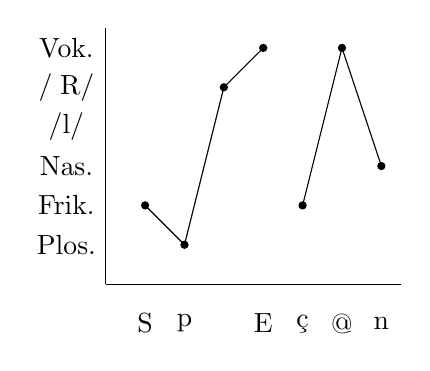
\begin{tikzpicture}[scale=0.5]
			\draw[black] (-1,0) -- (6.5,0) ; % x axis
			\draw[black] (-1,0) -- (-1,6.5); % y axis
			\node at (-2,1) {Plos.};
			\node at (-2,2) {Frik.};
			\node at (-2,3) {Nas.};
			\node at (-2,4) {\textipa{/l/}};
			\node at (-2,5) {\textipa{/\;R/}};
			\node at (-2,6) {Vok.};
			\draw[black] (0,2) -- (1,1) -- (2,5) -- (3,6);
			\draw[black] (4,2) -- (5,6) -- (6,3);
			\node at (0,-1) {\textipa{S}};
			\node at (1,-1) {\textipa{p}};
			\node at (2,-1) {\textipa{\textscr}};
			\node at (3,-1) {\textipa{E}};
			\node at (4,-1) {\textipa{\c{c}}};
			\node at (5,-1) {\textipa{@}};
			\node at (6,-1) {\textipa{n}};
			\fill (0,2) circle [radius=3pt];
			\fill (1,1) circle [radius=3pt];
			\fill (2,5) circle [radius=3pt];
			\fill (3,6) circle [radius=3pt];
			\fill (4,2) circle [radius=3pt];
			\fill (5,6) circle [radius=3pt];
			\fill (6,3) circle [radius=3pt];
			\end{tikzpicture}}
	\end{figure}
\end{minipage}
\begin{minipage}{.05\textwidth}
	\hfill
\end{minipage}
\begin{minipage}{.3\textwidth}
	\begin{figure}
		\centering
		\scalebox{.7}{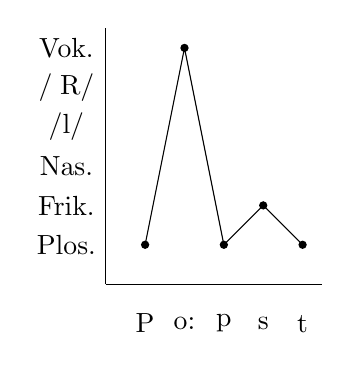
\begin{tikzpicture}[scale=0.5]
			\draw[black] (-1,0) -- (4.5,0) ; % x axis
			\draw[black] (-1,0) -- (-1,6.5); % y axis
			\node at (-2,1) {Plos.};
			\node at (-2,2) {Frik.};
			\node at (-2,3) {Nas.};
			\node at (-2,4) {\textipa{/l/}};
			\node at (-2,5) {\textipa{/\;R/}};
			\node at (-2,6) {Vok.};
			\draw[black] (0,1) -- (1,6) -- (2,1) -- (3,2) -- (4,1);
			\node at (0,-1) {\textipa{P}};
			\node at (1,-1) {\textipa{o:}};
			\node at (2,-1) {\textipa{p}};
			\node at (3,-1) {\textipa{s}};
			\node at (4,-1) {\textipa{t}};
			\fill (0,1) circle [radius=3pt];
			\fill (1,6) circle [radius=3pt];
			\fill (2,1) circle [radius=3pt];
			\fill (3,2) circle [radius=3pt];
			\fill (4,1) circle [radius=3pt];
			\end{tikzpicture}}
	\end{figure}
\end{minipage}
\begin{minipage}{.3\textwidth}
	\begin{figure}
		\centering
		\scalebox{.7}{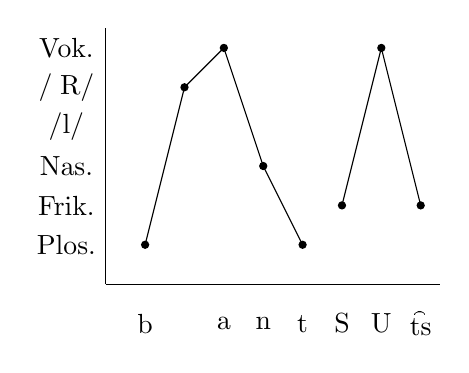
\begin{tikzpicture}[scale=0.5]
			\draw[black] (-1,0) -- (7.5,0) ; % x axis
			\draw[black] (-1,0) -- (-1,6.5); % y axis
			\node at (-2,1) {Plos.};
			\node at (-2,2) {Frik.};
			\node at (-2,3) {Nas.};
			\node at (-2,4) {\textipa{/l/}};
			\node at (-2,5) {\textipa{/\;R/}};
			\node at (-2,6) {Vok.};
			\draw[black] (0,1) -- (1,5) -- (2,6) -- (3,3) -- (4,1);
			\draw[black] (5,2) -- (6,6) -- (7,2);
			\node at (0,-1) {\textipa{b}};
			\node at (1,-1) {\textipa{\textscr}};
			\node at (2,-1) {\textipa{a}};
			\node at (3,-1) {\textipa{n}};
			\node at (4,-1) {\textipa{t}};
			\node at (5,-1) {\textipa{S}};
			\node at (6,-1) {\textipa{U}};
			\node at (7,-1) {\textipa{\t{ts}}};
			\fill (0,1) circle [radius=3pt];
			\fill (1,5) circle [radius=3pt];
			\fill (2,6) circle [radius=3pt];
			\fill (3,3) circle [radius=3pt];
			\fill (4,1) circle [radius=3pt];
			\fill (5,2) circle [radius=3pt];
			\fill (6,6) circle [radius=3pt];
			\fill (7,2) circle [radius=3pt];
			\end{tikzpicture}}
	\end{figure}
\end{minipage}


\end{frame}
%%%%%%%%%%%%%%%%%%%%%%%%%%%%%%%%%

\begin{frame}
\frametitle{Lösungen}

\begin{minipage}{.27\textwidth}
\centering
\scalebox{0.75}{
	\begin{forest} MyP edges, [,phantom
  [$\sigma$
		[O
			[x[\textipa{S}]]
			[x[\textipa{t}]]
		]
	[R
		[N
			[x[\textipa{\textsci}]]
		]
		[K
			[x[\textipa{m}]]
		]
	]]
	[$\sigma$
		[O]
	[R
		[N
			[x[\textipa{@}]]
		]
		[K
			[x[\textipa{n.}]]
		]
	]
	]
	[$\sigma$
		[O
			[x[\textipa{f}]]
		]
	[R
		[O
			[x[\textipa{a}]]
		]
		[K
			[X[\textipa{\ng}]]
		]
	]
	] ]
\end{forest}
}
\end{minipage}
\begin{minipage}{.1\textwidth}
	\hfill
\end{minipage}
%
\begin{minipage}{.45\textwidth}
\centering
\scalebox{.75}
{\begin{forest}
MyP edges, [, phantom
[$ \sigma $
	[O
		[x[\textipa{P}]]
	]
	[R
		[N
		[x[\textipa{a}]]
		]
		[K
		[x[\textipa{p}]]
		]
	]
]
[$ \sigma $
	[O
		[x[\textipa{S}]]
		[x[\textipa{t}]]
	]
	[R
		[N
		[x[\textipa{a}]]
		]
		[K
		[x[\textipa{n}]]
		[x[\textipa{\t{ts}}]]
		]
	]
]
[$ \sigma $
	[O
		[x[\textipa{h}]]
	]
	[R
		[N
		[x[\textipa{a}]]
		]
		[K
		[x[\textipa{l}]]
		]
	]
]
[$ \sigma $
	[O
		[x[t]]
	]
	[R	
		[N
		[x[\textipa{\textturna}]]
		]
	]
]
]
\end{forest}
}
\end{minipage}

\begin{minipage}{.3\textwidth}
		\begin{figure}
		\centering
		\scalebox{.7}{
		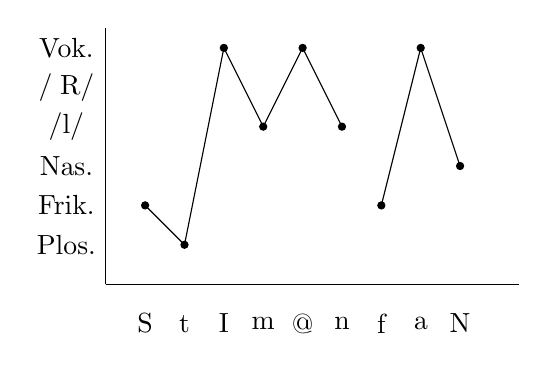
\begin{tikzpicture}[scale=0.5]
	\draw[black] (-1,0) -- (9.5,0) ; % x axis
	\draw[black] (-1,0) -- (-1,6.5); % y axis
	\node at (-2,1) {Plos.};
	\node at (-2,2) {Frik.};
	\node at (-2,3) {Nas.};
	\node at (-2,4) {\textipa{/l/}};
	\node at (-2,5) {\textipa{/\;R/}};
	\node at (-2,6) {Vok.};
	\draw[black] (0,2) -- (1,1) -- (2,6) -- (3,4) -- (4,6) -- (5,4);
	\draw[black] (6,2) -- (7,6) -- (8,3);
	\node at (0,-1) {\textipa{S}};
	\node at (1,-1) {\textipa{t}};
	\node at (2,-1) {\textipa{I}};
	\node at (3,-1) {\textipa{m}};
	\node at (4,-1) {\textipa{@}};
	\node at (5,-1) {\textipa{n}};
	\node at (6,-1) {\textipa{f}};
	\node at (7,-1) {\textipa{a}};
	\node at (8,-1) {\textipa{N}};
	\fill (0,2) circle [radius=3pt];
	\fill (1,1) circle [radius=3pt];
	\fill (2,6) circle [radius=3pt];
	\fill (3,4) circle [radius=3pt];
	\fill (4,6) circle [radius=3pt];
	\fill (5,4) circle [radius=3pt];
	\fill (6,2) circle [radius=3pt];
	\fill (7,6) circle [radius=3pt];
	\fill (8,3) circle [radius=3pt];
			\end{tikzpicture}}
	\end{figure}
\end{minipage}
\begin{minipage}{.15\textwidth}
	\hfill
\end{minipage}
\begin{minipage}{.4\textwidth}
	\begin{figure}
		\centering
		\scalebox{.7}{
			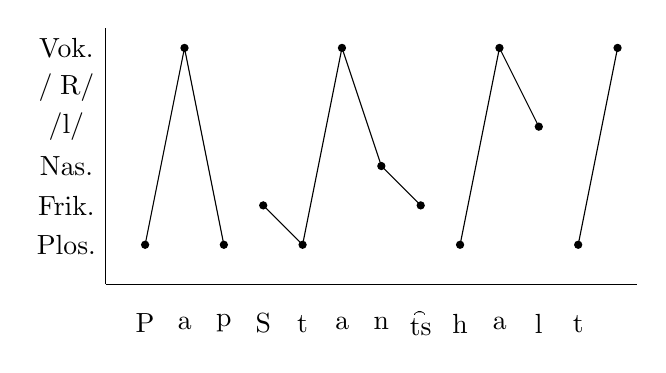
\begin{tikzpicture}[scale=0.5]
			\draw[black] (-1,0) -- (12.5,0) ; % x axis
			\draw[black] (-1,0) -- (-1,6.5); % y axis
			\node at (-2,1) {Plos.};
			\node at (-2,2) {Frik.};
			\node at (-2,3) {Nas.};
			\node at (-2,4) {\textipa{/l/}};
			\node at (-2,5) {\textipa{/\;R/}};
			\node at (-2,6) {Vok.};
			\draw[black] (0,1)--(1,6)--(2,1);
			\draw[black](3,2)--(4,1)--(5,6)--(6,3)--(7,2);
			\draw[black](8,1)--(9,6)--(10,4);
			\draw[black](11,1)--(12,6);
			\fill (0,1) circle [radius=3pt];
			\fill (1,6) circle [radius=3pt];
			\fill (2,1) circle [radius=3pt];
			\fill (3,2) circle [radius=3pt];
			\fill (4,1) circle [radius=3pt];
			\fill (5,6) circle [radius=3pt];
			\fill (6,3) circle [radius=3pt];
			\fill (7,2) circle [radius=3pt];
			\fill (8,1) circle [radius=3pt];
			\fill (9,6) circle [radius=3pt];
			\fill (10,4) circle [radius=3pt];
			\fill (11,1) circle [radius=3pt];
			\fill (12,6) circle [radius=3pt];
			\node at (0,-1){\textipa{P}};
			\node at (1,-1){\textipa{a}};
			\node at (2,-1){\textipa{p}};
			\node at (3,-1){\textipa{S}};
			\node at (4,-1){\textipa{t}};
			\node at (5,-1){\textipa{a}};
			\node at (6,-1){\textipa{n}};
			\node at (7,-1){\textipa{\t{ts}}};
			\node at (8,-1){\textipa{h}};
			\node at (9,-1){\textipa{a}};
			\node at (10,-1){\textipa{l}};
			\node at (11,-1){\textipa{t}};
			\node at (12,-1){\textipa{\textturna}};
			\end{tikzpicture}}
	\end{figure}
\end{minipage}

\end{frame}

%%%%%%%%%%%%%%%%%%%%%%%%%%
\begin{frame}
\frametitle{Lösungen}
	
	\begin{minipage}{.4\textwidth}
	\centering
	\scalebox{.75}
	{\begin{forest} MyP edges, [, phantom
	[$ \sigma $
		[O
			[x[m]]
		]
		[R
			[N
				[x[\textipa{\textsci}]]
			]
			[K
				[x[\textipa{t}]]
			]
		]
	]
	[$ \sigma $
		[O]
		[R
			[N
			[x[\textipa{a}]]
			]
			[K
			[x[\textipa{k}]]
			]
		]
	]
	[$ \sigma $
		[O
			[x[\textipa{P}] ]
		]
		[R
			[N
			[x[\textipa{E}]]
			]
			[K
			[x[\textipa{s}] ]
			]
		]
	]
	[$ \sigma $
		[O]
		[R
			[N
			[x[\textipa{\textschwa}]]
			]
			[K
				[x[\textipa{n}]]
			]
		]
	]
	]
	\end{forest}}
	\end{minipage}
	\begin{minipage}{.1\textwidth}
		\hfill
	\end{minipage}
	\begin{minipage}{.4\textwidth}
		\centering
		\scalebox{.75}{
		\begin{forest} MyP edges [, phantom
		[$ \sigma $
			[O
			[x[\textipa{b}]]
			]
			[R
				[N
					[x[\textipa{i:}, name=i]]
					[x, name=x]
					[x[\textipa{\textturna}]]
				]
			]
		]
		[$ \sigma $
			[O
				[x[\textipa{d}]]
			]
			[R
				[N
					[x[\textipa{E}]]
				]
				[K
					[x[\textipa{k}]]
					[x[\textipa{l}]]
				]
			] 
		]
	]
	\draw[black] (x.south)--(i.north);
		\end{forest}
	}
	\end{minipage}

\begin{minipage}{.3\textwidth}
	\begin{figure}
		\centering
		\scalebox{.7}{
	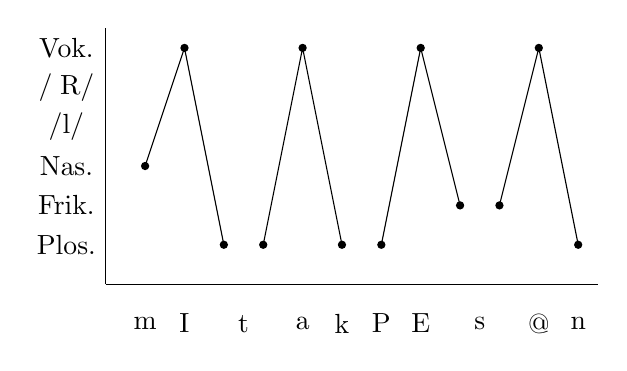
\begin{tikzpicture}[scale=0.5]
	\draw[black] (-1,0) -- (11.5,0) ; % x axis
	\draw[black] (-1,0) -- (-1,6.5); % y axis
	\node at (-2,1) {Plos.};
	\node at (-2,2) {Frik.};
	\node at (-2,3) {Nas.};
	\node at (-2,4) {\textipa{/l/}};
	\node at (-2,5) {\textipa{/\;R/}};
	\node at (-2,6) {Vok.};
	\draw[black] (0,3) -- (1,6) -- (2,1);
	\draw[black] (3,1) -- (4,6) -- (5,1);
	\draw[black] (6,1) -- (7,6) -- (8,2);
	\draw[black] (9,2) -- (10,6) -- (11,1);
	\node at (0,-1) {\textipa{m}};
	\node at (1,-1) {\textipa{I}};
	\node at (2.5,-1) {\textipa{t}};
	\node at (4,-1) {\textipa{a}};
	\node at (5,-1) {\textipa{k}};
	\node at (6,-1) {\textipa{P}};
	\node at (7,-1) {\textipa{E}};
	\node at (8.5,-1) {\textipa{s}};
	\node at (10,-1) {\textipa{@}};
	\node at (11,-1) {\textipa{n}};
	\fill (0,3) circle [radius=3pt];
	\fill (1,6) circle [radius=3pt];
	\fill (2,1) circle [radius=3pt];
	\fill (3,1) circle [radius=3pt];
	\fill (4,6) circle [radius=3pt];
	\fill (5,1) circle [radius=3pt];
	\fill (6,1) circle [radius=3pt];
	\fill (7,6) circle [radius=3pt];
	\fill (8,2) circle [radius=3pt];
	\fill (9,2) circle [radius=3pt];
	\fill (10,6) circle [radius=3pt];
	\fill (11,1) circle [radius=3pt];
	\end{tikzpicture}}
	\end{figure}
\end{minipage}
\begin{minipage}{.2\textwidth}
	\hfill
\end{minipage}
\begin{minipage}{.3\textwidth}
	\begin{figure}
		\centering
		\scalebox{.7}{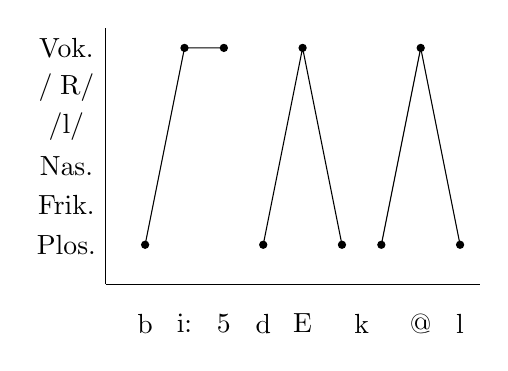
\begin{tikzpicture}[scale=0.5]
	\draw[black] (-1,0) -- (8.5,0) ; % x axis
	\draw[black] (-1,0) -- (-1,6.5); % y axis
	\node at (-2,1) {Plos.};
	\node at (-2,2) {Frik.};
	\node at (-2,3) {Nas.};
	\node at (-2,4) {\textipa{/l/}};
	\node at (-2,5) {\textipa{/\;R/}};
	\node at (-2,6) {Vok.};
	\draw[black] (0,1) -- (1,6) -- (2,6);
	\draw[black] (3,1) -- (4,6) -- (5,1);
	\draw[black] (6,1) -- (7,6) -- (8,1);
	\node at (0,-1) {\textipa{b}};
	\node at (1,-1) {\textipa{i:}};
	\node at (2,-1) {\textipa{5}};
	\node at (3,-1) {\textipa{d}};
	\node at (4,-1) {\textipa{E}};
	\node at (5.5,-1) {\textipa{k}};
	\node at (7,-1) {\textipa{@}};
	\node at (8,-1) {\textipa{l}};
	\fill (0,1) circle [radius=3pt];
	\fill (1,6) circle [radius=3pt];
	\fill (2,6) circle [radius=3pt];
	\fill (3,1) circle [radius=3pt];
	\fill (4,6) circle [radius=3pt];
	\fill (5,1) circle [radius=3pt];
	\fill (6,1) circle [radius=3pt];
	\fill (7,6) circle [radius=3pt];
	\fill (8,1) circle [radius=3pt];
	\end{tikzpicture}}
	\end{figure}
\end{minipage}
\end{frame}

}
%%%%%%%%%%%%%%%%%%%%%%%%%%%%%%%%%%%%%%%%%%%%%%%%%%%%%%%%%%%%%%
\subsection{Silbengelenk}
\iftoggle{toc}{
\frame{
\frametitle{~}
\begin{multicols}{2}
	\tableofcontents[currentsection]
\end{multicols}	
}
}
%%%%%%%%%%%%%%%%%%%%%%%%%%%%%%%%%%

\begin{frame}
\frametitle{Silbengelenk}


\begin{minipage}{.63\textwidth}

\begin{itemize}
	\item \textbf{ambisyllabischer Konsonant}
	
	\item[]
	\item Ein Konsonant,\\
               der zugleich \textbf{zu zwei Silben} gehört. 
	
	\item[]
	\item Nur \textbf{eine X Position} (nur eine Zeiteinheit, vgl. echte Geminaten)
	
\end{itemize}
\end{minipage}
%
\begin{minipage}{.35\textwidth}
%%%%%%%%%%%%%%
%%% Forestset Syllables

\newbox\foreststrutbox
\setbox\foreststrutbox=\hbox to 0pt{\phantom{\forestOve{standard node}{content}}}
\def\foreststrut{\copy\foreststrutbox}
\forestset{
GP1/.style 2 args={
for n={1}{baseline},
s sep=0pt, l sep=0pt,
for descendants={
l sep=0pt, l={#1},
anchor=base,calign=first,child anchor=north,
inner xsep=1pt,inner ysep=2pt,outer sep=0pt,s sep=0pt,
},
delay={
if content={}{phantom}{for children={no edge}},
for tree={
if content={O}{tier=OR}{},
if content={R}{tier=OR}{},
if content={N}{tier=N}{},
if content={x}{
tier=x,content={$\times$},outer xsep={#2},
for tree={calign=center},
for descendants={content format={\foreststrut\forestoption{content}}},
before drawing tree={outer xsep=0pt,delay={typeset node}},
s sep=4pt
}{},
},
},
before drawing tree={where content={}{parent anchor=center,child anchor=center}{}},
},
GP1/.default={5ex}{8.0pt},
associate/.style={%
tikz+={\draw(!)--(!#1);}},
spread/.style={
before drawing tree={tikz+={\draw[dotted](!)--(!#1);}}},
govern/.style={
before drawing tree={tikz+={\draw[->](!)--(!#1);}}},
p-govern/.style={
before drawing tree={tikz+={\draw[->](.north) to[out=150,in=30] (!#1.north);}}},
no p-govern/.style={
before drawing tree={tikz+={\draw[->,loosely dashed](.north) to[out=150,in=30] (!#1.north);}}},
encircle/.style={before drawing tree={circle,draw,inner sep=0pt}},
fen/.style={pin={[font=\footnotesize,inner sep=1pt,pin edge=<-]10:\textsc{Fen}}},
el/.style={content=\textsc{\textbf{##1}}},
head/.style={content=\textsc{\textbf{\underline{##1}}}},
llap/.style={
tikz+={%
\edef\forest@temp{\noexpand\node[\option{node options},
anchor=base east,at=(.base east)]}%
\forest@temp{#1\phantom{\option{environment}}};
}
},
rlap/.style={
tikz+={%
\edef\forest@temp{\noexpand\node[\option{node options},
anchor=base west,at=(.base west)]}%
\forest@temp{\phantom{\option{environment}}#1};
}
},
}
%%%%%%%%%%%%%

\footnotesize
\centering
\begin{forest} MyP edges, GP1 [
  [$\sigma$
    [O
    	[x
    		[\textipa{t}]
    	]
    ]
    [R
    	[N
    		[x
    			[\textipa{I}]
    		]
    	]  		
    	[K 
    		[x, name=x
    			[\textipa{k}]
    		]
    	]
    ]
  ]
  [$\sigma$
    [O, name=onset 
    ]
    [R
    	[N
    		[x
    			[\textipa{@}]
    		]
    	]
    	[K [x[\textipa{n}]]]]
  ]  
]
{
\draw[black] (x.north)--(onset.south);
}
\end{forest}

\end{minipage}

\end{frame}



%%%%%%%%%%%%%%%%%%%%%%%%%%%%%%%%%%

\begin{frame}
%\frametitle{Silbengelenk}

\begin{minipage}{.35\textwidth}
%%%%%%%%%%%%%%
%%% Forestset Syllables

\newbox\foreststrutbox
\setbox\foreststrutbox=\hbox to 0pt{\phantom{\forestOve{standard node}{content}}}
\def\foreststrut{\copy\foreststrutbox}
\forestset{
GP1/.style 2 args={
for n={1}{baseline},
s sep=0pt, l sep=0pt,
for descendants={
l sep=0pt, l={#1},
anchor=base,calign=first,child anchor=north,
inner xsep=1pt,inner ysep=2pt,outer sep=0pt,s sep=0pt,
},
delay={
if content={}{phantom}{for children={no edge}},
for tree={
if content={O}{tier=OR}{},
if content={R}{tier=OR}{},
if content={N}{tier=N}{},
if content={x}{
tier=x,content={$\times$},outer xsep={#2},
for tree={calign=center},
for descendants={content format={\foreststrut\forestoption{content}}},
before drawing tree={outer xsep=0pt,delay={typeset node}},
s sep=4pt
}{},
},
},
before drawing tree={where content={}{parent anchor=center,child anchor=center}{}},
},
GP1/.default={5ex}{8.0pt},
associate/.style={%
tikz+={\draw(!)--(!#1);}},
spread/.style={
before drawing tree={tikz+={\draw[dotted](!)--(!#1);}}},
govern/.style={
before drawing tree={tikz+={\draw[->](!)--(!#1);}}},
p-govern/.style={
before drawing tree={tikz+={\draw[->](.north) to[out=150,in=30] (!#1.north);}}},
no p-govern/.style={
before drawing tree={tikz+={\draw[->,loosely dashed](.north) to[out=150,in=30] (!#1.north);}}},
encircle/.style={before drawing tree={circle,draw,inner sep=0pt}},
fen/.style={pin={[font=\footnotesize,inner sep=1pt,pin edge=<-]10:\textsc{Fen}}},
el/.style={content=\textsc{\textbf{##1}}},
head/.style={content=\textsc{\textbf{\underline{##1}}}},
llap/.style={
tikz+={%
\edef\forest@temp{\noexpand\node[\option{node options},
anchor=base east,at=(.base east)]}%
\forest@temp{#1\phantom{\option{environment}}};
}
},
rlap/.style={
tikz+={%
\edef\forest@temp{\noexpand\node[\option{node options},
anchor=base west,at=(.base west)]}%
\forest@temp{\phantom{\option{environment}}#1};
}
},
}
%%%%%%%%%%%%%

\footnotesize
\centering
\begin{forest} MyP edges, GP1 [
  [$\sigma$
    [O
    	[x
    		[\textipa{k}]
    	]
    	[x	[\textipa{l}]]
    ]
    [R
    	[N
    		[x
    			[\textipa{I}]
    		]
    	]  		
    	[K 
    		[x, name=x
    			[\textipa{N}]
    		]
    	]
    ]
  ]
  [$\sigma$
    [O, name=onset
    ]
    [R
    	[N
    		[x
    			[\textipa{@}]
    		]
    	]
    	[K [x[\textipa{n}]]]]
  ]  
]
{
\draw[black] (x.north)--(onset.south);
}
\end{forest}

\end{minipage}
%
\begin{minipage}{.63\textwidth}

\begin{itemize}
	\item \textbf{In der Schreibung} werden Silbengelenke häufig mit Doppelkonsonanten markiert (aber nicht immer!)
	
	\ea der \textipa{[\t{tS}Et]} \vs ich \textipa{[\t{tS}Et@]}\\
	\pause der Cha\alertred{t} \vs ich cha\alertred{tt}e
	\z
	\ea
        abkli\alertred{ng}en, zwi\alertred{sch}en
        \z
% abklingngen, zwischschen durch ästhetisches Prinzip verboten

\pause
	
	\item \textbf{Silbengelenke kommen nach betonten ungespannten Vokalen vor. }
	
	Ungespannte betonte Vokale kommen nicht in offenen Silben vor.

	\item Linear: \textbf{Markierung} durch Punkt
	
	  \ea
          \textipa{[Pap.klI\.N@n]}
          \z
	
\end{itemize}

\end{minipage}

\end{frame}



%%%%%%%%%%%%%%%%%%%%%%%%%%%%%%%%%%
%%%%%%%%%%%%%%%%%%%%%%%%%%%%%%%%%%
\subsection{Silbifizierung}
\iftoggle{toc}{
\frame{
\frametitle{~}
\begin{multicols}{2}
	\tableofcontents[currentsection]
\end{multicols}	
}
}
%%%%%%%%%%%%%%%%%%%%%%%%%%%%%%%%%%

\begin{frame}
\frametitle{Silbifizierung}

\begin{itemize}
	\item Silbifizierung, Syllabierung $:=$ in Silben einteilen
	\item[]
	\item Wie würden Sie folgende Lautsequenzen silbifizieren?:

	  \ea
          ata, odo, eke
          \z

\pause

	\item Ein einziger intervokalischer Konsonant wird immer als Silbenanlaut silbifiziert (universelles Prinzip: \textbf{Onset-Maximierung})
	
	
\end{itemize}

\begin{block}{Onsetmaximierung}
Bilde zuerst den größtmöglichen Silbenanlaut;\\ dann bilde den Silbenauslaut \citep[218]{Hall00a}
\end{block}

\end{frame}



%%%%%%%%%%%%%%%%%%%%%%%%%%%%%%%%%%

\begin{frame}
%\frametitle{Silbifizierung}

\begin{block}{Onsetmaximierung}
Bilde zuerst den größtmöglichen Silbenanlaut; dann bilde den Silbenauslaut \citep[218]{Hall00a}
\end{block}


\begin{itemize}
	\item Onset-Maximierung herleitbar aus:
	\begin{enumerate}
		\item Silbenanlautgesetz (CV häufiger als V), und
		\item Silbenauslautgesetz (CVC$^{n} >$ CVC$^{n+1}$)
	\end{enumerate}

\pause
	\item Silbifizierung nicht über Morphemgrenzen hinweg! 
	\item Ausnahme: Suffixe mit vokalischem Onset:
	
	  \ea
          kind\#isch: \textipa{[kIn.dIS]}
          \z
	
	  \ea
          kind\#lich: \textipa{[kInt.lI\c{c}]}
          \z
          
     \item \# := Morphemgrenze

% Wenn man Morphmgrenzenbedingung weglassen würde, ergäbe sich Bra. ndschutz

% rek.nen vs. re.gnen
	
\end{itemize}

\end{frame}


\iftoggle{uebung}{

%%%%%%%%%%%%%%%%%%%%%%%%%%%%%%%%%%
%%%%%%%%%%%%%%%%%%%%%%%%%%%%%%%%%%
%\subsection{Übung}
%\iftoggle{toc}{
%\frame{
%\frametitle{~}
%\begin{multicols}{2}
%	\tableofcontents[currentsection]
%\end{multicols}	
%}
%}
%%%%%%%%%%%%%%%%%%%%%%%%%%%%%%%%%%

\begin{frame}
\frametitle{Übung}

\begin{itemize}
	\item Was bedeutet die Annahme des Sonoritätsprinzips und der Onset-Maximierung für die folgenden Beispielwörter:
	
	  \ea
          Fabrik, Imker, neblig, Falter, regnen
          \z
	
\pause
\ea
\textipa{[fa:.b\textscr Ik]}, \textipa{[PIm.k5]}, \textipa{[ne:.blI\c{c}]}, \textipa{[fal.t5]}, \textipa{[\textscr e:.gn@n]}\\
	Koda: *Obstruent vor Sonorant\\
	Onset: *Sonorant vor Obstruent
\z
	
	\item Welche Prinzipien bzw. Regularitäten werden verletzt bei:
	\eal
	\ex \textipa{[PE.b@]}
	\ex \textipa{[PEb.@]}
	\ex \textipa{[PEp.@]}
	\ex \textipa{[PEp.b@]}
        \zl

\end{itemize}

\end{frame}



%%%%%%%%%%%%%%%%%%%%%%%%%%%%%%%%%%



\begin{frame}
%\frametitle{Übung}

\begin{itemize}
	\item Silbifizieren Sie folgende Segmentsequenzen in zwei Schritten
	\begin{itemize}
		\item Onsetmaximierungsprinzip
		\item Sonoritätsprinzip
	\end{itemize}

Stellen Sie fest, ob alle Silben wohlgeformt sind. Falls nicht, benennen Sie die Verletzungen
	
\ea
\textipa{[o:tlIN5mSplag\textscr e:hOn]}
\z

% Otlingamsplagrehon

\ea
Blumentopferde
\z
% blu.men.to.pfer.de

%\ea
%Urinstinkt
%\z	
	\item Geben Sie die standarddeutsche phonetische Transkription des Wortes \ab{Stahltische} inklusive der Silbenstruktur (mit X-Skelettschicht) an. Ermitteln Sie die Kriterien, die bei der Silbifizierung wirken.
	
\end{itemize}

% ' Stahl , tische     Hauptbetonung auf Stahl, Nebenbetonung auf Tische


\end{frame}
}


%%%%%%%%%%%%%%%%%%%%%%%%%%%%%%%%%%
%%%%%%%%%%%%%%%%%%%%%%%%%%%%%%%%%%
\subsection{Exkurs: Akzent}
\iftoggle{toc}{
\frame{
\frametitle{~}
\begin{multicols}{2}
	\tableofcontents[currentsection]
\end{multicols}	
}
}
%%%%%%%%%%%%%%%%%%%%%%%%%%%%%%%%%%

\begin{frame}
\frametitle{Exkurs: Akzent}

\begin{itemize}
	\item Silben können \textbf{betont} oder \textbf{unbetont} sein, d.\,h. sie können einen Akzent tragen oder nicht
	\item[]

\begin{block}{Akzent}
\textbf{Auditiver Eindruck der Prominenz eines Vokals} gegenüber einem anderen durch (relational, nicht absolut!):
\begin{itemize}
	\item Lautstärke
	\item Dauer
	\item Höhere Tonlage
	\item Ausgeprägtere Artikulationsbewegungen
\end{itemize}
\end{block}	 
	
	\item[]
	\item Man unterscheidet zwischen \textbf{Wort-} und \textbf{Satzakzent} (engl. \emph{stress} und \emph{accent})

\end{itemize}

\end{frame}



%%%%%%%%%%%%%%%%%%%%%%%%%%%%%%%%%%%
%%%%%%%%%%%%%%%%%%%%%%%%%%%%%%%%%%
%\subsubsection{Exkurs: Wortakzent}
%\frame{
%\begin{multicols}{2}
%\frametitle{~}
%	\tableofcontents[currentsection]
%\end{multicols}
%}
%%%%%%%%%%%%%%%%%%%%%%%%%%%%%%%%%%

\begin{frame}
\frametitle{Exkurs: Wortakzent}

\begin{itemize}
	\item Was scheint die häufigste Betonung im Deutschen zu sein?
	
	  \ea
          Mutter, Männer, Autos, Hühner, Lehrer, Kinder, alle \dots
          \z
	
\pause
	\textbf{betont-unbetont (Trochäus)}
	
	\item Ausnahmen (die je nach Theorie verschieden erklärt werden):
	
	\eal 
	\ex \textipa{["f\textscr aU]}
	\ex \textipa{[mu.\textprimstress zi:k]}
	\ex \textipa{["le:.b@n.d@]}
	\ex \textipa{\originalTeX [pa.pa."g\t{aI}]}
	\ex \textipa{[f\t{E5}.\textprimstress Pa5.b\t{aI}.t@n]}
	\zl

\end{itemize}

\end{frame}



%%%%%%%%%%%%%%%%%%%%%%%%%%%%%%%%%%%
%%%%%%%%%%%%%%%%%%%%%%%%%%%%%%%%%%
%\subsubsection{Exkurs: Satzakzent}
%\frame{
%\begin{multicols}{2}
%\frametitle{~}
%	\tableofcontents[currentsection]
%\end{multicols}
%}
%%%%%%%%%%%%%%%%%%%%%%%%%%%%%%%%%%

\begin{frame}
\frametitle{Exkurs: Satzakzent}

\begin{itemize}
	\item In einem Satz können betonte Silben \textbf{noch weiter hervorgehoben} werden (dabei meist durch die Tonhöhe):
	
	\eal 
	\ex Géstern hat BAyern gewónnen.
	\ex GÉStern hat Báyern gewónnen.
	\ex Géstern hat Báyern geWONnen.
	\zl
	\item Die prominenteste Silbe im Satz wird meist mit \textbf{Großbuchstaben} dargestellt, sie trägt den Satzakzent

	\item Durch diese Akzentuierung wird das gesamte Wort
hervorgehoben \ras \textbf{Fokus des Satzes} (\gqq{Informationsstruktur})
	
\end{itemize}

\end{frame}



%%%%%%%%%%%%%%%%%%%%%%%%%%%%%%%%%%%
%%%%%%%%%%%%%%%%%%%%%%%%%%%%%%%%%%
%\subsubsection{Exkurs: Intonation}
%\frame{
%\begin{multicols}{2}
%\frametitle{~}
%	\tableofcontents[currentsection]
%\end{multicols}
%}
%%%%%%%%%%%%%%%%%%%%%%%%%%%%%%%%%%

\begin{frame}
\frametitle{Exkurs: Intonation}

\begin{block}{Intonation}
Tonhöhenverlauf (\gqq{Melodie}) einer Äußerung
\end{block}

\begin{itemize}
	\item \textbf{Satztypen} können mittels Intonation unterschieden werden.
	
	\item Sprechen Sie die folgenden Äußerungen mit fallender und steigender Intonation
	\eal 
	\ex Heute gewinnen die Bayern.
	\ex Schon Schluss.
        \zl
\pause
	\textbf{Aussage-} \vs \textbf{Interrogativsatz}	
	
\end{itemize}

\end{frame}



%%%%%%%%%%%%%%%%%%%%%%%%%%%%%%%%%%

\begin{frame}
%\frametitle{Exkurs: Intonation}

\begin{itemize}
	\item Ambige ($\approx$ mehrdeutige) Sätze können mittels Intonation \gs{durch die sog. Hutkontur} \textbf{disambiguiert} werden: 
	
	  \ea
          Alle Studenten haben die Klausur nicht bestanden.
          \z
        \eal
	\ex Es ist nicht der Fall, dass alle Studenten die Klausur bestanden haben. \hfill $\lsem \neg \forall \rsem$
	\ex Für alle Studenten gilt, dass sie die Klausur nicht bestanden haben. \hfill $\lsem \forall \neg \rsem$
        \zl
\pause 

\ea
/Alle Studenten haben die Klausur  nicht\textbackslash\ bestanden.
\z
\eal
\ex Es ist nicht der Fall, dass alle Studenten die Klausur bestanden haben. \hfill $\lsem \neg \forall \rsem$
	\zl

\end{itemize}

\end{frame}


\iftoggle{hausaufgabe}{
	
	\subsection{Hausaufgabe}
	\iftoggle{toc}{
		\frame{
			\frametitle{~}
			\begin{multicols}{2}
				\tableofcontents[currentsection]
			\end{multicols}	
		}
	}
	
	
%%%%%%%%%%%%%%%%%%%%%%%%%%%%%%%%%%
\begin{frame}%[allowframebreaks]
	\frametitle{Hausaufgabe}
\begin{itemize}
			
	\item[1.] Geben Sie eine phonetische Tranksription der folgenden Wörter nach der \gqq{Standardaussprache} an, zeichnen Sie dabei die Silbestruktur nach dem Konstituentenmodell und mit der Skelettschicht, und geben Sie die Sonoritätsprofile an.
		
	\begin{block}{Sonoritätshierarchie (Zur Erinnerung)}
		Vokal $>$ \textipa{/\textscr /} $>$ \textipa{/l/} $>$ Nasal $>$ Frikativ $>$ Plosiv \\
		$x > y :=$ $x$ ist sonorer als $y$
	\end{block}
		
		\eal 
		\ex Stimmenfang
		\ex Mittagessen
		\ex Bierdeckel
		\zl
\end{itemize}
\end{frame}

\begin{frame}
\begin{itemize}
	\item[2.] Silbifizieren Sie folgende Segmentsequenzen in zwei Schritten
	\begin{itemize}
		\item Onsetmaximierungsprinzip
		\item Sonoritätsprinzip
	\end{itemize}
	
	Stellen Sie fest, ob alle Silben wohlgeformt sind. Falls nicht, benennen Sie die Verletzungen	
	\ea
	Urinstinkt
	\z	
	\item[3.] Geben Sie die standarddeutsche phonetische Transkription des Wortes \ab{Stahltische} inklusive der Silbenstruktur (mit X-Skelettschicht) an. Ermitteln Sie die Kriterien, die bei der Silbifizierung wirken.
	
	\item[4.] Geben Sie die Gründe an, warum die folgenden Wörter aus phonetisch/ phonologischen Gründen im Deutschen nicht möglich sind:
	
	\eal
	\ex[*]{\textipa{['Napl.O:t]}}
	\ex[*]{\textipa{[a\;R.'tUng]}}
	\zl
	
\end{itemize}

\end{frame}
	
}


%%%%%%%%%%%%%%%%%%%%%%%%%%%% Lösungen %%%%%%%%%%%%%%%%%%%%%%%%%%%%%%

\iftoggle{loesung}{
	
	\subsection{Hausaufgabe}
	\iftoggle{toc}{
		\frame{
			\frametitle{~}
			\begin{multicols}{2}
				\tableofcontents[currentsection]
			\end{multicols}	
		}
	}
	
	
%%%%%%%%%%%%%%%%%%%%%%%%%%%%%%%%%%
\begin{frame}%[allowframebreaks]
	\frametitle{Hausaufgabe}
	\begin{itemize}
			
		\item[1.] Geben Sie eine phonetische Tranksription der folgenden Wörter nach der \gqq{Standardaussprache} an, zeichnen Sie dabei die Silbestruktur nach dem Konstituentenmodell und mit der Skelettschicht, und geben Sie die Sonoritätsprofile an.
			
		\begin{block}{Sonoritätshierarchie (Zur Erinnerung)}
			Vokal $>$ \textipa{/\textscr /} $>$ \textipa{/l/} $>$ Nasal $>$ Frikativ $>$ Plosiv \\
			$x > y :=$ $x$ ist sonorer als $y$
		\end{block}
			
			\eal 
			\ex Stimmenfang
			\ex Mittagessen
			\ex Bierdeckel
			\zl
			
	\end{itemize}
\end{frame}

\begin{frame}

%\begin{minipage}{.35\textwidth}
			%%%%%%%%%%%%%%
%%% Forestset Syllables

\newbox\foreststrutbox
\setbox\foreststrutbox=\hbox to 0pt{\phantom{\forestOve{standard node}{content}}}
\def\foreststrut{\copy\foreststrutbox}
\forestset{
GP1/.style 2 args={
for n={1}{baseline},
s sep=0pt, l sep=0pt,
for descendants={
l sep=0pt, l={#1},
anchor=base,calign=first,child anchor=north,
inner xsep=1pt,inner ysep=2pt,outer sep=0pt,s sep=0pt,
},
delay={
if content={}{phantom}{for children={no edge}},
for tree={
if content={O}{tier=OR}{},
if content={R}{tier=OR}{},
if content={N}{tier=N}{},
if content={x}{
tier=x,content={$\times$},outer xsep={#2},
for tree={calign=center},
for descendants={content format={\foreststrut\forestoption{content}}},
before drawing tree={outer xsep=0pt,delay={typeset node}},
s sep=4pt
}{},
},
},
before drawing tree={where content={}{parent anchor=center,child anchor=center}{}},
},
GP1/.default={5ex}{8.0pt},
associate/.style={%
tikz+={\draw(!)--(!#1);}},
spread/.style={
before drawing tree={tikz+={\draw[dotted](!)--(!#1);}}},
govern/.style={
before drawing tree={tikz+={\draw[->](!)--(!#1);}}},
p-govern/.style={
before drawing tree={tikz+={\draw[->](.north) to[out=150,in=30] (!#1.north);}}},
no p-govern/.style={
before drawing tree={tikz+={\draw[->,loosely dashed](.north) to[out=150,in=30] (!#1.north);}}},
encircle/.style={before drawing tree={circle,draw,inner sep=0pt}},
fen/.style={pin={[font=\footnotesize,inner sep=1pt,pin edge=<-]10:\textsc{Fen}}},
el/.style={content=\textsc{\textbf{##1}}},
head/.style={content=\textsc{\textbf{\underline{##1}}}},
llap/.style={
tikz+={%
\edef\forest@temp{\noexpand\node[\option{node options},
anchor=base east,at=(.base east)]}%
\forest@temp{#1\phantom{\option{environment}}};
}
},
rlap/.style={
tikz+={%
\edef\forest@temp{\noexpand\node[\option{node options},
anchor=base west,at=(.base west)]}%
\forest@temp{\phantom{\option{environment}}#1};
}
},
}
%%%%%%%%%%%%%

			\footnotesize
			\centering
		\begin{exe}
		\exi{(54)~a.}
			\begin{forest} MyP edges, GP1 [
				[$\sigma$
				[O [x [\textipa{S}]] [x [\textipa{t}]]]
				[R [N [x [\textipa{I}]]] [K [x, name=x [\textipa{m}]]]]
				]
				[$\sigma$
				[O, name=onset]
				[R [N [x [\textipa{@}]]] [K [x [\textipa{n}]]]]
				]
				[$\sigma$
				[O [x [\textipa{f}]]]
				[R [N [x [\textipa{a}]]] [K [x [\textipa{N}]]]]
				]
				]				
				{
					\draw[black] (x.north)--(onset.south);
				}
			\end{forest}
		
		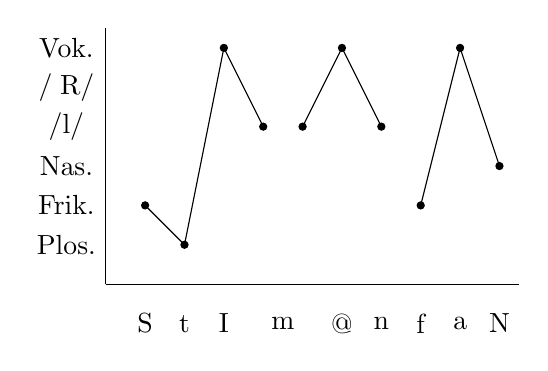
\begin{tikzpicture}[scale=0.5]
		\draw[black] (-1,0) -- (9.5,0) ; % x axis
		\draw[black] (-1,0) -- (-1,6.5); % y axis
		\node at (-2,1) {Plos.};
		\node at (-2,2) {Frik.};
		\node at (-2,3) {Nas.};
		\node at (-2,4) {\textipa{/l/}};
		\node at (-2,5) {\textipa{/\;R/}};
		\node at (-2,6) {Vok.};
		\draw[black] (0,2) -- (1,1) -- (2,6) -- (3,4);
		\draw[black] (4,4) -- (5,6) -- (6,4);
		\draw[black] (7,2) -- (8,6) -- (9,3);
		\node at (0,-1) {\textipa{S}};
		\node at (1,-1) {\textipa{t}};
		\node at (2,-1) {\textipa{I}};
		\node at (3.5,-1) {\textipa{m}};
		\node at (5,-1) {\textipa{@}};
		\node at (6,-1) {\textipa{n}};
		\node at (7,-1) {\textipa{f}};
		\node at (8,-1) {\textipa{a}};
		\node at (9,-1) {\textipa{N}};
		\fill (0,2) circle [radius=3pt];
		\fill (1,1) circle [radius=3pt];
		\fill (2,6) circle [radius=3pt];
		\fill (3,4) circle [radius=3pt];
		\fill (4,4) circle [radius=3pt];
		\fill (5,6) circle [radius=3pt];
		\fill (6,4) circle [radius=3pt];
		\fill (7,2) circle [radius=3pt];
		\fill (8,6) circle [radius=3pt];
		\fill (9,3) circle [radius=3pt];
		\end{tikzpicture}
\end{exe}
\end{frame}

\begin{frame}			
%\end{minipage}%
%\begin{minipage}{.35\textwidth}
	\footnotesize
	\centering
	\begin{exe}
	\exi{(54)~b.}
	\begin{forest} MyP edges, GP1 [
	[$\sigma$
	[O [x [\textipa{m}]]] 
	[R [N [x [\textipa{I}]]] [K [x, name=x1 [\textipa{t}]]]]
	]
	[$\sigma$
	[O, name=onset1]
	[R [N [x [\textipa{a}]]] [K [x [\textipa{k}]]]]
	]
	[$\sigma$
	[O [x [\textipa{P}]]]
	[R [N [x [\textipa{E}]]] [K [x, name=x2 [\textipa{s}]]]]
	]
	[$\sigma$
	[O, name=onset2]
	[R [N [x [\textipa{@}]]] [K [x [\textipa{n}]]]]
	]
	]
	{
		\draw[black] (x1.north)--(onset1.south);
		\draw[black] (x2.north)--(onset2.south);
	}
	\end{forest}

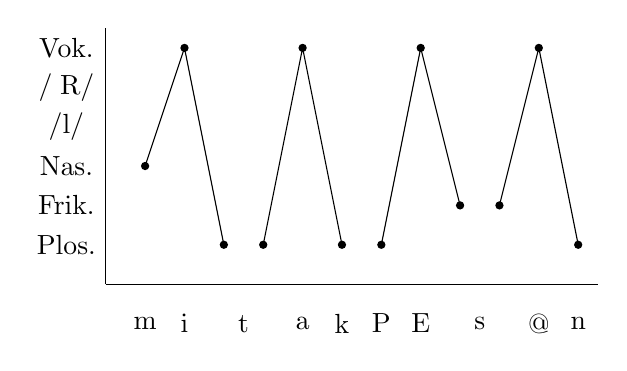
\begin{tikzpicture}[scale=0.5]
\draw[black] (-1,0) -- (11.5,0) ; % x axis
\draw[black] (-1,0) -- (-1,6.5); % y axis
\node at (-2,1) {Plos.};
\node at (-2,2) {Frik.};
\node at (-2,3) {Nas.};
\node at (-2,4) {\textipa{/l/}};
\node at (-2,5) {\textipa{/\;R/}};
\node at (-2,6) {Vok.};
\draw[black] (0,3) -- (1,6) -- (2,1);
\draw[black] (3,1) -- (4,6) -- (5,1);
\draw[black] (6,1) -- (7,6) -- (8,2);
\draw[black] (9,2) -- (10,6) -- (11,1);
\node at (0,-1) {\textipa{m}};
\node at (1,-1) {\textipa{i}};
\node at (2.5,-1) {\textipa{t}};
\node at (4,-1) {\textipa{a}};
\node at (5,-1) {\textipa{k}};
\node at (6,-1) {\textipa{P}};
\node at (7,-1) {\textipa{E}};
\node at (8.5,-1) {\textipa{s}};
\node at (10,-1) {\textipa{@}};
\node at (11,-1) {\textipa{n}};
\fill (0,3) circle [radius=3pt];
\fill (1,6) circle [radius=3pt];
\fill (2,1) circle [radius=3pt];
\fill (3,1) circle [radius=3pt];
\fill (4,6) circle [radius=3pt];
\fill (5,1) circle [radius=3pt];
\fill (6,1) circle [radius=3pt];
\fill (7,6) circle [radius=3pt];
\fill (8,2) circle [radius=3pt];
\fill (9,2) circle [radius=3pt];
\fill (10,6) circle [radius=3pt];
\fill (11,1) circle [radius=3pt];
\end{tikzpicture}
\end{exe}
%\end{minipage}
	
\end{frame}

\begin{frame}

%\begin{minipage}{.35\textwidth}
	\footnotesize
	\centering
\begin{exe}
	\exi{(54)~c.}
	\begin{forest} MyP edges, GP1 [
	[$\sigma$
	[O [x [\textipa{b}]]]
	[R [N [x [\textipa{i}]] [x [\textipa{:}]]] [K [x [\textipa{5}]]]]
	]
	[$\sigma$
	[O [x [\textipa{d}]]]
	[R [N [x [\textipa{E}]]] [K [x, name=x [\textipa{k}]]]]
	]
	[$\sigma$
	[O, name=onset]
	[R [N [x [\textipa{@}]]] [K [x [\textipa{l}]]]]
	]
	]
	{
		\draw[black] (x.north)--(onset.south);
	}
	\end{forest}

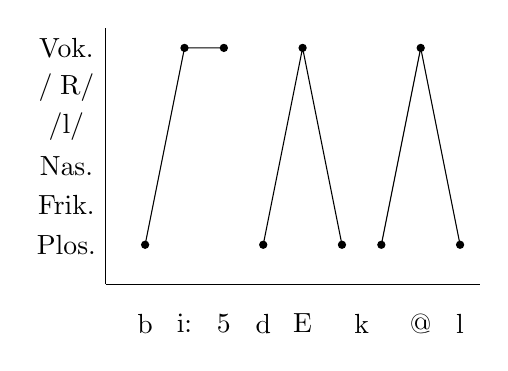
\begin{tikzpicture}[scale=0.5]
\draw[black] (-1,0) -- (8.5,0) ; % x axis
\draw[black] (-1,0) -- (-1,6.5); % y axis
\node at (-2,1) {Plos.};
\node at (-2,2) {Frik.};
\node at (-2,3) {Nas.};
\node at (-2,4) {\textipa{/l/}};
\node at (-2,5) {\textipa{/\;R/}};
\node at (-2,6) {Vok.};
\draw[black] (0,1) -- (1,6) -- (2,6);
\draw[black] (3,1) -- (4,6) -- (5,1);
\draw[black] (6,1) -- (7,6) -- (8,1);
\node at (0,-1) {\textipa{b}};
\node at (1,-1) {\textipa{i:}};
\node at (2,-1) {\textipa{5}};
\node at (3,-1) {\textipa{d}};
\node at (4,-1) {\textipa{E}};
\node at (5.5,-1) {\textipa{k}};
\node at (7,-1) {\textipa{@}};
\node at (8,-1) {\textipa{l}};
\fill (0,1) circle [radius=3pt];
\fill (1,6) circle [radius=3pt];
\fill (2,6) circle [radius=3pt];
\fill (3,1) circle [radius=3pt];
\fill (4,6) circle [radius=3pt];
\fill (5,1) circle [radius=3pt];
\fill (6,1) circle [radius=3pt];
\fill (7,6) circle [radius=3pt];
\fill (8,1) circle [radius=3pt];
\end{tikzpicture}

\end{exe}

\end{frame}
	
\begin{frame}
	\begin{itemize}
		\item[2.] Silbifizieren Sie folgende Segmentsequenzen in zwei Schritten
			\begin{itemize}
				\item Onsetmaximierungsprinzip
				\item Sonoritätsprinzip
			\end{itemize}
			
		Stellen Sie fest, ob alle Silben wohlgeformt sind. Falls nicht, benennen Sie die Verletzungen	
		\ea
		Urinstinkt
		\z
		
		\eal
		\ex \textipa{[Pu.\;RI.nStInkt]} (Onsetmaximierung)
		\ex \textipa{[Pu.\;RIn.(S)tInkt]} (Sonoritätsprinzip)
		\ex \textipa{[Pu5.PIn.stinkt]} (Silbifizierung)
		\zl 
		\item Die Silbifizierung erfolgt auf der Ebene des phonologischen Wortes. Daher werden die phonologischen Wörter \ab{ur-} und \ab{Instinkt} einzeln silbifiziert.
	
	\end{itemize}
\end{frame}


\begin{frame}
	\begin{itemize}	
		\item[3.] Geben Sie die standarddeutsche phonetische Transkription des Wortes \ab{Stahltische} inklusive der Silbenstruktur (mit X-Skelettschicht) an. Ermitteln Sie die Kriterien, die bei der Silbifizierung wirken.
			
		\end{itemize}
\end{frame}


\begin{frame}
	\begin{itemize}
					
		\item[4.] Geben Sie die Gründe an, warum die folgenden Wörter aus phonetisch/ phonologischen Gründen im Deutschen nicht möglich sind:
			
		\eal
		\ex[*]{\textipa{['Napl.O:t]}} Onset Maximierung \textipa{[pl]}, \textipa{[N]} steht am Wortanfang, \textipa{[O]} ist ungespannt und lang
		\ex[*]{\textipa{[a\;R.'tUng]}} Auslautverhärtung, regressive velarare nasale Assimilation, Knacklaut
		\zl
			
	\end{itemize}
		
\end{frame}
	
}


%%%%%%%%%%%%%%%%%%%%%%%%%%%%%%%%%%%
%%%%%%%%%%%%%%%%%%%%%%%%%%%%%%%%%%%
%\subsection{X}
%%\frame{
%%\frametitle{~}
%%	\tableofcontents[currentsection]
%%}


%%%%%%%%%%%%%%%%%%%%%%%%%%%%%%%%%%%
%\begin{frame}
%\frametitle{Y}
%
%\begin{itemize}
%	\item 
%
%\end{itemize}
%
%\end{frame}



%%%%%%%%%%%%%%%%%%%%%%%%%%%%%%%%%%%
%\begin{frame}
%\frametitle{Y}
%
%\begin{itemize}
%	\item 
%
%\end{itemize}
%
%\end{frame}



%%%%%%%%%%%%%%%%%%%%%%%%%%%%%%%%%%%
%%%%%%%%%%%%%%%%%%%%%%%%%%%%%%%%%%%
%\subsection{X}
%%\frame{
%%\frametitle{~}
%%	\tableofcontents[currentsection]
%%}


%%%%%%%%%%%%%%%%%%%%%%%%%%%%%%%%%%%
%\begin{frame}
%\frametitle{Y}
%
%\begin{itemize}
%	\item 
%
%\end{itemize}
%
%\end{frame}




